\chapter{Testing}

\section{Test Plan}

\begin{landscape}
\subsection{Original Outline Plan}

\begin{center}
    \begin{tabular}{|p{2cm}|p{5cm}|p{5cm}|p{4cm}|}
        \hline
        \textbf{Test Series} & \textbf{Purpose of Test Series} & \textbf{Testing Strategy} & \textbf{Strategy Rationale}\\ \hline
         1 & Test the flow of control between the user interfaces & Top-down testing & Without a correct flow of control between the user interfaces, the application will not be useable therefore I must test the flow of control.  \\ \hline
	2 & Test validation of data input is detected & Bottom-up testing & The program needs to be tested on its reliablity and so using this strategy, I will be able to find out \\ \hline
	3 & Test information input is stored in the correct place & Black box testing & Information needs to be stored in the correct place to prevent confusion thus making the application more usable \\ \hline
	4 & Test algorithms to make sure that the output is correct & White box testing & Output needs to be correct for the application to be useable therefore I can find out by using this strategy \\ \hline
	5 & Test that the system fufils the specification & Acceptance testing & Get an overall idea if the new system is usable and meets the requirements of my client  \\ \hline
	6 & Test database has referential integrity & Integration testing &Find out whether the manipulation of the database is reliable  \\ \hline
    \end{tabular}
\end{center}

\subsection{Changes to Outline Plan}

\begin{center}
    \begin{tabular}{|p{2cm}|p{5cm}|p{5cm}|p{4cm}|}
        \hline
        \textbf{Test Series} & \textbf{Purpose of Test Series} & \textbf{Testing Strategy} & \textbf{Strategy Rationale}\\ \hline
	4 & Test algorithms \textbf{and SQL statements} to make sure that the output is correct & White box testing & Output needs to be correct for the application to be useable therefore I can find out by using this strategy \\ \hline
    \end{tabular}
\end{center}

\subsection{Original Detailed Plan}
The original details plan below looks different than the one in the Design section as I have formatted the plan below so that each test data has its own row.

I have not tested the rows that are in grey due to changes in my program.

\begin{center}
    \begin{longtable}{|p{1.5cm}|p{2.5cm}|p{2.5cm}|p{2cm}|p{2cm}|p{2cm}|p{2cm}|p{2cm}|}
        \hline
        \textbf{Test Series} & \textbf{Purpose of Test} & \textbf{Test Description} & \textbf{Test Data} & \textbf{Test Data Type (Normal/ Erroneous/ Boundary)} & \textbf{Expected Result} & \textbf{Actual Result} & \textbf{Evidence}\\ \hline
        \rowcolor{gray}1.01 & Test 'Change password' button functions correctly & Should direct user to change password interface  & Click Change password button & Normal & Change password interface should be displayed &  &  \\ \hline
         \rowcolor{gray}*1.02 & Test Cancel button functions correctly on change password interface & Should redirect user to login screen  & Click Cancel button on change password interface & Normal & Change password interfact should close &  &  \\ \hline
         \rowcolor{gray}*1.03 & Test interactive table functions correctly & Should direct user to the order details from the table selected  & Click on occupied table & Normal & Table  information screen should be displayed &  &  \\ \hline
        \rowcolor{gray} *1.04 & Test unoccupied table functions correctly & Should direct user to 'add details to table'  interface  & Click on unoccupied table & Normal & 'Add details to table' interface should be displayed & Add details to table displayed - expected &  \\ \hline
        \rowcolor{gray} *1.05 & Test Table information screen, add button functions correctly & Should direct user to add item  interface  & Click Add on table information screen & Normal & Add item interface should be displayed & Add item interface displayed - expected  &  \\ \hline
        \rowcolor{gray} *1.06 & Test table information screen, delete function correctly & Should change colour of delete button and red box will appear to indiciate deletion for items  & Click Delete button & Normal & Delete button should change colour and red boxes should appear next to each order item &  &  \\ \hline
        \rowcolor{gray} *1.07 & Test 'Change password' button functions correctly & Should direct user to change password interface  & Click Change password button & Normal & Change password interface should be displayed &  &  \\ \hline
         \rowcolor{gray}*1.08 & Test back arrow button functions correctly on table information screen & Should direct user to main screen & Click back arrow button & Normal & User redirected back to main screen should be displayed &  &  \\ \hline
        1.09 & Test 'Manage Bookings' button functions correctly on main screen & Should direct user to Manage Bookings interface  & Click Manage Bookings & Normal & Manage Bookings interface should be displayed & Manage Bookings interface displayed - expected  & \ref{fig:Test1} on page \pageref{fig:Test1} \\ \hline
        1.10 & Test Add Booking button functions correctly on Manage Bookings interface & Should direct user to create booking interface  & Click Add Booking button & Normal & Create booking interface should be displayed & Create booking interface displayed - expected & \ref{fig:Test2} on page \pageref{fig:Test2}  \\ \hline
        \rowcolor{gray} *1.11 & Test Cancel button functions correctly on create booking interface & Should redirect user to Manage Bookings interface  & Click Cancel button & Normal & User should be redirected to Manage Bookings interface &  &  \\ \hline
        \rowcolor{gray} *1.12 & Test back arrow on manage bookings interface functions correctly & Should redirect user to main screen  & Click Change back arrow button & Normal & Main screen should be displayed &  &  \\ \hline
        1.13 & Test Delete Booking button on Manage Bookings screen & Should direct user to delete bookings display interface  & Click Delete button & Normal & Delete bookings display should be displayed  &Delete bookings layout displayed - expected  & \ref{fig:Test3} on page \pageref{fig:Test3}  \\ \hline
        \rowcolor{gray} *1.14 & Test back arrow button functions correctly on bookings display screen & Should redirect user to Manage Bookings interface  & Click back arrow button & Normal & User should be redirected to Manage Bookings interface &  &  \\ \hline
       \rowcolor{gray} * 2.01 & Verify password entered & The field cannot be left blank  & (Nothing), Treem & Erroneous, Normal & Error, Accepted &  &  \\ \hline
        \rowcolor{gray} *2.01.01 & Verify new password entered at change password screen & The field cannot be left blank  & (Nothing), PineTree & Erroneous, Normal & Error, Accepted &  &  \\ \hline
        \rowcolor{gray} *2.02 & Verify retype new password entered at change password screen & The field cannot be left blank  & (Nothing), PineTree & Erroneous, Normal & Error, Accepted &  &  \\ \hline
        \rowcolor{gray} *2.03 & Verify old password entered at change password screen & The field cannot be left blank  & (Nothing) ,Treem & Erroneous, Normal & Error, Accepted &  &  \\ \hline
        2.04 & Verify Number of people entered at 'assign customer to table' & User inputs nothing  & (Nothing)& Erroneous & Error&Nothing - expected  & \ref{fig:Test4} on page \pageref{fig:Test4} \\ \hline
        2.04.01 & Verify Number of people entered at 'assign customer to table' &  User inputs value  & 3 &  Normal & Accepted &  Accept input - expected &  \\ \hline
        2.04.02 & Verify Number of people entered at 'assign customer to table' &  User inputs value  & pigs&  Erroneous &  Error &Can only enter numbers - expected due to regular expression  &  \\ \hline
        2.05 & Verify ItemID entered at 'add item to order' interface &  User inputs vnothing  & (Nothing) & Erroneous & Error/ nothing & No changes - expected  &  \\ \hline
        2.05.01 & Verify ItemID entered at 'add item to order' interface &  User inputs value  & 3 &Normal& Accepted & Accepted   &  \\ \hline
        2.05.02 & Verify ItemID entered at 'add item to order' interface &  User inputs value  & 9552 &Erroneous& Error& Only allowed to input 3 digits  &  \\ \hline
        2.06 & Verify First Name entered at 'enter booking details' interface &  User inputs nothing  & (Nothing) & Erroneous & Error & Add booking did not proceed after clicking add booking - expected &  \\ \hline
	2.06.01 & Verify First Name entered at 'enter booking details' interface & User inputs name  & Milly & Normal&Accepted& Milly was accepted and booking proceeded - expected  &  \\ \hline
	2.06.02 & Verify First Name entered at 'enter booking details' interface & User inputs name  & 63 & Erroneous &Error & Could not enter numbers - expected due to regular expression  &  \\ \hline
        2.07 & Verify Last Name entered at 'enter booking details' interface & User inputs name  & (Nothing)& Erroneous& Error&Add booking did not proceeed after clicking add booking  &  \\ \hline
        2.07.01 & Verify Last Name entered at 'enter booking details' interface & User inputs name  &  Milk&  Normal& Accepted &Milk was accepted and booking proceeded - expected  &  \\ \hline
        2.07.02 & Verify Last Name entered at 'enter booking details' interface & User inputs name  & 2 & Erroneous &Error & Could not enter numbers - expected due to regular expression  &  \\ \hline
        2.08 & Verify Telephone Number entered at 'enter booking details'' interface & User inputs nothing  & (Nothing)& Errorneous &Error &Add booking did not proceed - expected  &  \ref{fig:Test12} on page \pageref{fig:Test12}  \\ \hline
        2.08.01 & Verify Telephone Number entered at 'enter booking details'' interface & User inputs number  & 01523 859372 &Normal&Accepted&Add booking did proceed - expected  &  \\ \hline
        2.08.02 & Verify Number entered at 'enter booking details'' interface & User inputs number  &  014829&Boundary &Error & Add booking did not proceed - expected  &  \ref{fig:Test13} on page \pageref{fig:Test13} \\ \hline
       \rowcolor{gray}  *2.09 & Verify Table Number entered at 'enter booking details' interface & User inputs number  & (Nothing)& Erroneous& Error&  &  \\ \hline
       \rowcolor{gray}  *2.09.01 & Verify Table Number entered at 'enter booking details' interface & User inputs number  & 7 & Normal&Accepted &  &  \\ \hline
       \rowcolor{gray}  *2.09.02 & Verify Table Number entered at 'enter booking details' interface & User inputs number  & Hey & Erroneous &Error &  &  \\ \hline
        2.10 & Verify Number Of People entered at 'enter booking details' interface & User inputs nothing & (Nothing)& Erroneous& Error& Add booking did not proceed - expected  &  \\ \hline
        2.10.01 & Verify Number Of People entered at 'enter booking details' interface & User inputs number & 3& Normal& Accepted& Add booking proceeded - expected &  \\ \hline
        2.10.02 & Verify Number Of People entered at 'enter booking details' interface &User inputs number  &  Lisa & Erroneous & Error & Could not enter letters - expected due to regular expression &  \\ \hline
      \rowcolor{gray}   *2.11 & Verify Date entered at 'enter booking details' interface & User inputs date  & (Nothing& Erroneous& Error&  &  \\ \hline
       \rowcolor{gray}  *2.11.01& Verify Date entered at 'enter booking details' interface & User inputs date    & 06/05/13 &  Normal&Accepted&  &  \\ \hline
        \rowcolor{gray} *2.11.02& Verify Date entered at 'enter booking details' interface & User inputs date    & Homer& Erroneous& Error&  &  \\ \hline
        \rowcolor{gray} *2.11.03& Verify Date entered at 'enter booking details' interface & User inputs date    &032/63/153 & Erroneous& Error&  &  \\ \hline
      \rowcolor{gray}   *2.12 & Verify Time entered at 'enter booking details' interface & User inputs time   & (Nothing)& Erroneous& Error&  &  \\ \hline
	2.12.01 & Verify Time entered at 'enter booking details' interface & User inputs time  &18:12&Normal& Accepted& Add booking proceeded - expected &  \\ \hline
       \rowcolor{gray}  *2.12.02 & Verify Time entered at 'enter booking details' interface & User inputs time  & Bart& Erroneous &Error &  &  \\ \hline
       \rowcolor{gray}  *2.12.03 & Verify Time entered at 'enter booking details' interface & User inputs time  & 53:62 &  Erroneous &  Error &  &  \\ \hline
      \rowcolor{gray}   *3.01 & Verify all table details entered are added to relevant database tables & Information should be added to the correct fields in customer, order and orderitem  tables. If necessary reservation table  & customer information, order information, orderitem information, if necessary reservation table & Normal &Added to customer, order and orderitem table. If necessary reservation table  & & \\ \hline
        3.02 & Verify that all details entered at 'enter booking details' interface are added to the booking database & All of the information should be added to the correct field in the booking table  & Booking information & Normal & Relevent details added to booking table & All details have been added to relevent database tables - expected &  \\ \hline
       \rowcolor{gray}  *4.01 & Verify password changed & Password should not successfully change if length is not bigger than 4 and old password does not match input old password   & Try changing password with incorrect input and length of 2 new password,&Error& & \\ \hline
      \rowcolor{gray}   *4.01.01 & Verify password changed & Password should not successfully change if length is not bigger than 4 and old password does not match input old password   &Try changing password with new password having length of 2&Error& & \\ \hline
      \rowcolor{gray}   *4.01.02 & Verify password changed & Password should not successfully change if length is not bigger than 4 and old password does not match input old password   &  Try changing password with correct input and correct length&Accepted  & & \\ \hline
       \rowcolor{gray}  *4.02 & Verify add item function works correctly & Entering MenuID will return information based on that ID & Enter ID &  Normal & Return all information based on the ID  & & \\ \hline
        4.03 & Verify Total price calculation functions correctly & Adds up all items prices together to get a total & Enter items to order &  Normal & Calculates the total price based on items entered  & Total doesnt update - unexpected & \ref{fig:Test10} on page \pageref{fig:Test10} \\ \hline
	4.04 & Check bookings displayed on correct day & Should display all bookings that match with system date & Create a range of bookings that have different dates & Normal& Displays correct bookings & & \\ \hline
         5.01 & Verify program fulfills the specification & Run through the program, testing all aspects to make sure the meet the objectives in the specification & Enter information in all places required input &  Normal & Program fulfils specification  & Can run through program without any problems, some minor objectives were not met such as having clickable tables (I have radio buttons instead). & \\ \hline
	 \rowcolor{gray}*6.01 & Verify menu item name updates in case an item is mistakenly spelt & Check  the item name is updated in all records that it appears in & Update name of a menu item (Wate to Water) & Normal & Wate should change to Water & & \\ \hline
	 \rowcolor{gray}*6.02 & Verify menu item price updates in case an item is mistakenly priced & Check the price of the item is updated in all records the item appears in & Update price of a menu item (0.060) to (0.60) & Normal & Price should change to 0.60 & & \\ \hline






    \end{longtable}
\end{center}
	I have removed some tests under 2.09, 2.11 and 2.12 due to changes in my program which made it impossible to have the wrong input in terms of erroneous and boundary inputs. For example, test 2.09 was to verify the table number inputted was valid, I have made my program so now the user can only select tables which exist through a combo box. As for tests 2.11 and 2.12, the user is forced into using the correct times/dates format. I set the minimum date for QDateEdit to be the system date which would mean the user will not be able to input boundary data (make a booking for yesterday).

\subsection{Changes to Detailed Plan}

\begin{center}
    \begin{longtable}{|p{1.5cm}|p{2.5cm}|p{2.5cm}|p{2cm}|p{2cm}|p{2cm}|p{2cm}|p{2cm}|}
        \hline
        \textbf{Test Series} & \textbf{Purpose of Test} & \textbf{Test Description} & \textbf{Test Data} & \textbf{Test Data Type (Normal/ Erroneous/ Boundary)} & \textbf{Expected Result} & \textbf{Actual Result} & \textbf{Evidence}\\ \hline
       1.15 & Test Add Item on 'Item Menu' menu bar & Check if Add Item layout is displayed after clicking on Add Item & Click on Add Item & Normal & Add Item layout displayed & Add Item layout displayed - expected &  \\ \hline
       1.16 & Test Delete Item on 'Item Menu' menu bar & Check if Delete Item layout is displayed after clicking on Delete Item & Click on Delete Item & Normal & Delete Item layout displayed & Delete Item layout is displayed &  \\ \hline
       1.17 & Test Update Item Price on 'Item Menu' menu bar & Check if Update Item Price layout is displayed after clicking on Update Item Price & Click on Update Item Price & Normal & Update Item Price layout displayed & Update Item Price layout displayed - expected & \\ \hline
       1.18 & Test Add Booking on 'Bookings' menu bar & Check if Add Booking layout is displayed after clicking on Add Booking & Click on Add Booking & Normal & Add Booking layout displayed &Add Booking layout displayed - expected &  \\ \hline
       1.19 & Test Delete Booking on 'Bookings' menu bar & Check if Delete Booking layout is displayed after clicking on Delete Booking & Click on Delete Booking & Normal & Delete Booking layout displayed & Delete Booking layout displayed - expected & \\ \hline
       1.20 & Test Update Booking on 'Bookings' menu bar & Check if Update Booking layout is displayed after clicking on Update Booking & Click on Update Booking & Normal & Update Booking layout displayed & Update Booking layout displayed - expected &  \\ \hline
       1.21 & Test 'Search Order' on tool bar & Check if Search Order layout is displayed after clicking on Search Order & Click on Search Order & Normal & Search Order layout displayed & Search Order layout displayed - expected & \ref{fig:searchOrder} on page \pageref{fig:searchOrder} \\ \hline
       1.22 & Test 'View Bookings' on tool bar & Check if View Bookings layout is displayed after clicking on View Bookings & Click on View Bookings & Normal & View Bookings layout displayed & View Bookings layout displayed - expected &  \\ \hline
       1.23 & Test 'View Customers' on tool bar & Check if View Customers layout is displayed after clicking on View Customers & Click on View Customers & Normal & View Customers layout displayed &View Customers layout displayed - expected &  \\ \hline
       1.24 & Test 'View Dishes' on tool bar & Check View Dishes layout is displayed after clicking on View Dishes & Click on View Dishes & Normal & View Dishes layout displayed & View Dishes layout displayed - expected & \\ \hline
       1.25 & Test 'View Drinks' on tool bar & Check if View Drinks layout is displayed after clicking on View Drinks & Click on View Drinks & Normal & View Drinks layout displayed & View Drinks layout displayed - expected &  \\ \hline
       1.26 & Test 'Main Screen' on tool bar & Check if Main Screen is displayed after clicking on 'Main Screen' & Click on Main Screen from Search Order layout & Normal & Main Screen layout displayed & Main Screen layout displayed - expected &  \\ \hline
       1.27 & Test table radio buttons on main screen & Check if dialog box shows after clicking on Select Table & Choose an unoccupied table and click Select Table & Normal & Assign customer dialog box shows & Assign customer dialog box is shown - expected & \\ \hline
       1.28 & Test Assign customer layout & Check if manage order box shows after clicking on Create (after filling in required field) & Click on Create & Normal & Relevent manage order dialog box shows & Relevent manage order dialog box is shown - expected &  \\ \hline
       1.28.01 & Test Assign customer layout & Check if manage order box shows after clicking on Select & Click on Select & Normal & Relevent manage order dialog box shows & Relevent manage order dialog box is shown &  \\ \hline
       1.29 & Test Add button on manage order box & Check if Add Item To Order box shows after clicking on Add & Click on Add & Normal & Add Item To Order dialog box shows & Add Item To Order dialog box is shown - expected &  \\ \hline
       1.30 & Test Delete button on manage order box & Check Delete Item Off Order box shows after clicking on Delete & Click on Delete & Normal & Delete Item Off Order dialog box shows & Delete Item Off Order dialog box is shown &  \\ \hline
       1.31 & Test Finish button on manage order box & Check if Manage Order box closes after clicking on Finish & Click on Finish & Normal & Manage Order box closes & Manage Order box closes - expected &  \\ \hline
       1.32 & Test Invoice Preview button on manage order box & Check if the preview of the invoice box shows after clicking on Invoice Preview & Click on Invoice Preview & Normal & Invoice preview shows & Invoice shown - expected &  \ref{fig:Test7} on page \pageref{fig:Test7} \\ \hline
       1.33 & Test Print Invoice button on manage order box & Check if print option appear after clicking Print Invoice & Click on Print Invoice & Normal & Print options appear & Print options appeared - expected & \\ \hline
        2.04.03 & Verify Number of people entered at 'assign customer to table' & Check if user input is valid after clicking Create  & 0 &  Boundary &  Input not accepted &  Input was not accepted - expected  &  \\ \hline
        2.13 & Verify Item Name input at Add Item to Menu & Check if user input is valid after clicking Add Item assuming all other fields are filled with normal data  & Rice &  Normal &  Accepted & Item was successfully added  &  \\ \hline
        2.13.01 & Verify Item Name input at Add Item to Menu & Check if user input is valid after clicking Add Item assuming all other fields are filled with normal data  & (Nothing) & Erroneus & Error  &Item add unsuccessful - expected    & \ref{fig:Test11} on page \pageref{fig:Test11}  \\ \hline
        2.14 & Verify ItemID input at Update Item Price & Check if user input is valid after clicking Update Item assuming all other fields are filled with normal data  & 7 &  Normal &  Accepted & Price was successfully updated   &  \\ \hline
        2.14.01 & Verify ItemID input at Update Item Price & Check if user input is valid after clicking Update Item assuming all other fields are filled with normal data  & 0 &  Boundary & Error  &  Nothing happened - expected   &  \\ \hline
        2.15 & Verify Number Of People at Update Booking & Check if user input is valid after clicking Update Number Of People with a booking that exists  & 5 &  Normal &  Accepted & Booking updated - expected    &  \\ \hline
        2.15.01 & Verify Number Of People at Update Booking & Check if user input is valid after clicking Update Number Of People with a booking that exists  & 0 &  Boundary &  No changes will be made & Booking did not update - expected &  \\ \hline
	2.16 & Verify Item Name at Delete Item Off Menu & Check if user input is valid after clicking Delete Item for Item Name &  Nothing & Erroneous & Error(no chages will be made) & The process of deleting an item did not happen - expected & \\ \hline
	2.16.01 & Verify Item Name at Delete Item Off Menu & Check if user input is valid after clicking Delete Item for Item Name & Steak   &  Normal & Steak will be deleted & Steak was successfully deleted (removed from the displayed table widget) - expected & \\ \hline
	2.17 & Verify Item ID at Delete Item Off Menu & Check is user input is valid after clicking Delete Item for Item Name & 10(Steak which ive added again) & Normal & Record with Item ID 10 deleted & Item ID 10 was deleted (removed from the displayed table ) - expected & \\ \hline
	2.17.01 & Verify Item ID at Delete Item Off Menu & Check is user input is valid after clicking Delete Item for Item Name & (Nothing) & Erroneous & Error(no changes will be made) & The process of deleting an item did not happen - expected & \\ \hline
	2.17.02 & Verify Item ID at Delete Item Off Menu & Check is user input is valid after clicking Delete Item for Item Name & 645(There was not an item with itemID 645) & Boundary & Error(no changes will be made) & The process of deleting an item did not happen - expected & \\ \hline
	2.18 & Verify Booking ID at Delete Booking& Check is user input is valid &(Nothing )& Erroneous & Error(no changes will be made) & The process of deleting a booking did not happen - expected & \\ \hline
	2.18.01 & Verify Booking ID at Delete Booking& Check is user input is valid &888& Boundary & Error(no changes will be made) & There was not an error but the process of deleting a booking did not happen & \\ \hline
	2.18.02 & Verify Booking ID at Delete Booking& Check is user input is valid &18(Booking which ive added for testing purposes)& Normal & Booking deleted & Booking removed(Booking was removed from the displayed boking table) - expected  & \\ \hline


	3.03 & Check all details from the creation of a booking at Assign Customer to table is transferred & Check all correct details are transferred over to the Manage Order box & Click on Create after filling in fields correctly & Normal & All relevent details displayed & All relevent details transferred & \ref{fig:Test5} on page \pageref{fig:Test5}\\ \hline
	3.04 & Check all details from the selecting of a booking at Assign Customer to table is transferred & Check all correct details are transferred over to the Manage Order box & Click on Select after selecting a booking from combo box & Normal & All relevent details displayed & All relevent details transferred &\ref{fig:Test8} on page \pageref{fig:Test8}\\ \hline

	3.05 & Check all details from an order is transferred to invoice & Compare the order details to invoice details to make sure they are the same & Click on Invoice Preview & Normal & All relevent details displayed & All relevent details transferred & \ref{fig:Test7} on page \pageref{fig:Test7} \\ \hline
	3.06 & Booking added is stored in correct table & After successfully adding a booking, the booking should be displayed in table above & Add Booking & Normal & All relevent details displayed & All relevent details displayed in table above &\\ \hline
	3.07 & Customer added is stored in correct table & After successfully adding a booking, a customer record should be added to Customer table & Add Booking & Normal & All relevent details displayed & All relevant details added to table &\\ \hline
	3.08 & Item added to menu is stored in correct table & After successfully adding an item, an item record should be appear on  Items table & Add Booking & Normal & All relevent details displayed & New item appeared &\\ \hline
	4.03.01 & Verify Total price calculation algorithm is correct & Check that an algorithm adds up all items prices together to get a total & Check invoice preview to see total price &  Normal & Calculates the total price based on items ordered  & Correct total price - expected & \\ \hline
	4.05 & Check if the 'Increasing the quantity of an ordered item' algorithm works & A customer can order x more of an item - the quantity should therefore increase by x amount & Add an item initially then add 10 more if it &  Normal & Should expect quantity to be 11  & Quantity increased to 11 - expected & \ref{fig:Test6} on page \pageref{fig:Test6} \\ \hline
	4.06&Check if only drinks are displayed on View Drinks tool bar & After clicking View Drinks, a table should appear with only drinks in it&Click on View Drinks & Normal & Only items with ItemTypeID 2 appear & Drinks were only displayed - expected & \\ \hline
	4.07&Check if only dishes are displayed on View Dishes tool bar & After clicking View Dishes, a table should appear with only dishes in it&Click on View Dishes & Normal & Only items with ItemTypeID 1 appear & Dishes were only displayed & \\ \hline
           4.08 & Check search order function & Leave the booking field blank and click Search Order & (Nothing) &  Erroneous &  Error /empty table appear & Empty table appeared    &  \\ \hline
           4.08.01 & Check search order function & Enter a booking ID that doesn't exist and click Search Order & 93 &  Boundary &  Error / empty table appear &  Empty table appeared  &  \\ \hline
           4.08.02& Check search order function & Enter a booking ID that exists and click Search Order & 11 &  Normal &  A populated table appear & Correct table appeared   & \ref{fig:searchFunction} on page \pageref{fig:searchFunction} \\ \hline
	4.09 & Check Customer details entered are stored correctly & Input details using normal data & "Moe", "Iro", "15/04/2015", "17:30", " 5", "01639435231", (select table 1)  & Normal & A new customer record will be created with the details "Moe", "Iro" and "01639435231". & First Name and Last Name stored correctly - expected however, Telephone did not store correctly as it stored "1639435231" instead of "01639435231" &  \ref{fig:Test9} on page \pageref{fig:Test9}\\ \hline
	6.03 & Ensure order gets deleted when booking gets deleted & After deleting a booking, the order should be deleted with it.  & Delete a booking which has booking items   & Normal & Order should be deleted &Order(Booking items) has been deleted &\ref{fig:searchDeletedBooking} on page \pageref{fig:searchDeletedBooking} \\ \hline
	6.04 & Check if an item that does not exist is added to an order & Adding an item that does not exist from the manage order box  & Add Item ID 933 & Boundary & Nothing should happen as there isnt an item with an ID of 993 & No items were added& \\ \hline
	


    \end{longtable}
\end{center}
\end{landscape}

\section{Test Data}

\subsection{Original Test Data}

\begin{center}
    \begin{tabular}{|p{2cm}|p{3cm}|p{7cm}|}
        \hline
        \textbf{Test Number} & \textbf{Test Data} & \textbf{Justification for choice of test data}\\ \hline

	2.04.01 & 3 & Program must allow the correct input \\ \hline
	2.04.01 & pigs & Program must not  allow the wrong input, regular expression shouldn't allow letters to be inputted \\ \hline
	2.05 & (Nothing) &User could accidently try to proceed without entering anything which shouldn't be accepted by validation \\ \hline
	2.05.01 & 3 & Program must allow the correct input \\ \hline
	2.05.02 & 9552 & Program must not allow an erroneous input \\ \hline
	2.06 & (Nothing) &User could accidently try to proceed without entering anything which shouldn't be accepted by validation \\ \hline
	2.06.01 & 3 & Program must allow the correct input \\ \hline
	2.06.02 & 63 & Program must not  allow the wrong input, regular expression shouldn't allow numbers to be inputted \\ \hline
	2.07 & (Nothing) & User could accidently try to proceed without entering anything which shouldn't be accepted by validation \\ \hline
	2.07.01 & Milk & Program must allow the correct input \\ \hline
	2.07.02 & 2 & Program must not  allow the wrong input, regular expression shouldn't allow numbers to be inputted \\ \hline
	2.08 & (Nothing) &User could accidently try to proceed without entering anything which shouldn't be accepted by validation\\ \hline
	2.08.01 & 0152385972 & Program must allow the correct input (11 numbers) \\ \hline
	2.08.02 & 014829 & Program must not allow an invalid number (not 11 numbers) \\ \hline
	2.10 & (Nothing) & User could accidently try to proceed without entering anything which shouldn't be accepted by validation \\ \hline
	2.10.01 & 3 & Program must allow the correct input \\ \hline
	2.10.02 & 2 & Program must not allow the wrong input, regular expression shouldn't allow letters to be inputted \\ \hline


	

    \end{tabular}
\end{center}


\subsection{Changes to Test Data}

Some of the new test's test data will be included in the table below.

\begin{center}
    \begin{tabular}{|p{2cm}|p{3cm}|p{7cm}|}
        \hline
        \textbf{Test Number} & \textbf{Test Data} & \textbf{Justification for choice of test data}\\ \hline

	2.04.03 & 0 & Program should not allow 0 as it would not make sense if there was a booking for 0 people \\ \hline
	2.13 & Rice & Program must allow the correct input \\ \hline
	2.13.01 & (Nothing) &User could accidently try to proceed without entering anything which shouldn't be accepted by validation \\ \hline
	2.14 & 7 & Program must allow the correct input \\ \hline
	2.14.01 & 0 & Program must not allow 0 because it will not exist in the database \\ \hline
	2.15 & 5 & Program must allow the correct input  \\ \hline
	2.15.01 & 0 & Program should not allow 0 as it would not make sense if there was a booking for 0 people  \\ \hline
	2.16& (Nothing) & User could accidently try to proceed without entering anything which shouldn't be accepted by validation \\ \hline
	2.16.01 & Steak & Program must allow the correct input \\ \hline
	2.17 & 10(Steak) & Program must allow the correct input \\ \hline
	2.17.01& (Nothing) &User could accidently try to proceed without entering anything which shouldn't be accepted by validation \\ \hline
	2.17.02 & 645& Should allow the correct input but not do anything/error stating input is incorrect \\ \hline
	2.18& (Nothing) & User could accidently try to proceed without entering anything which shouldn't be accepted by validation \\ \hline
	2.18.01 & 888 & Should allow 888 as it is a valid input but not do anything as there is not a booking with an id of 888 in the current database used for testing \\ \hline
	2.18.02 & 18& Should allow the correct input but not do anything/error stating input is incorrect \\ \hline

	4.05 & Have an item with a quantity of 1 then add 10 more of it & I have chosen 1 as the initial quantity and the additional 10 because it will be very clear if the adding quantity algorithm works. \\ \hline

    \end{tabular}
\end{center}

\section{Annotated Samples}

\subsection{Actual Results}
The actual results for the tests can be found on the detailed plans, there is a seperate column for it named 'Actual Results'.

\subsection{Evidence}

\subsubsection{From main screen to manage bookings (Test 1.09)}

\begin{figure}[H]
    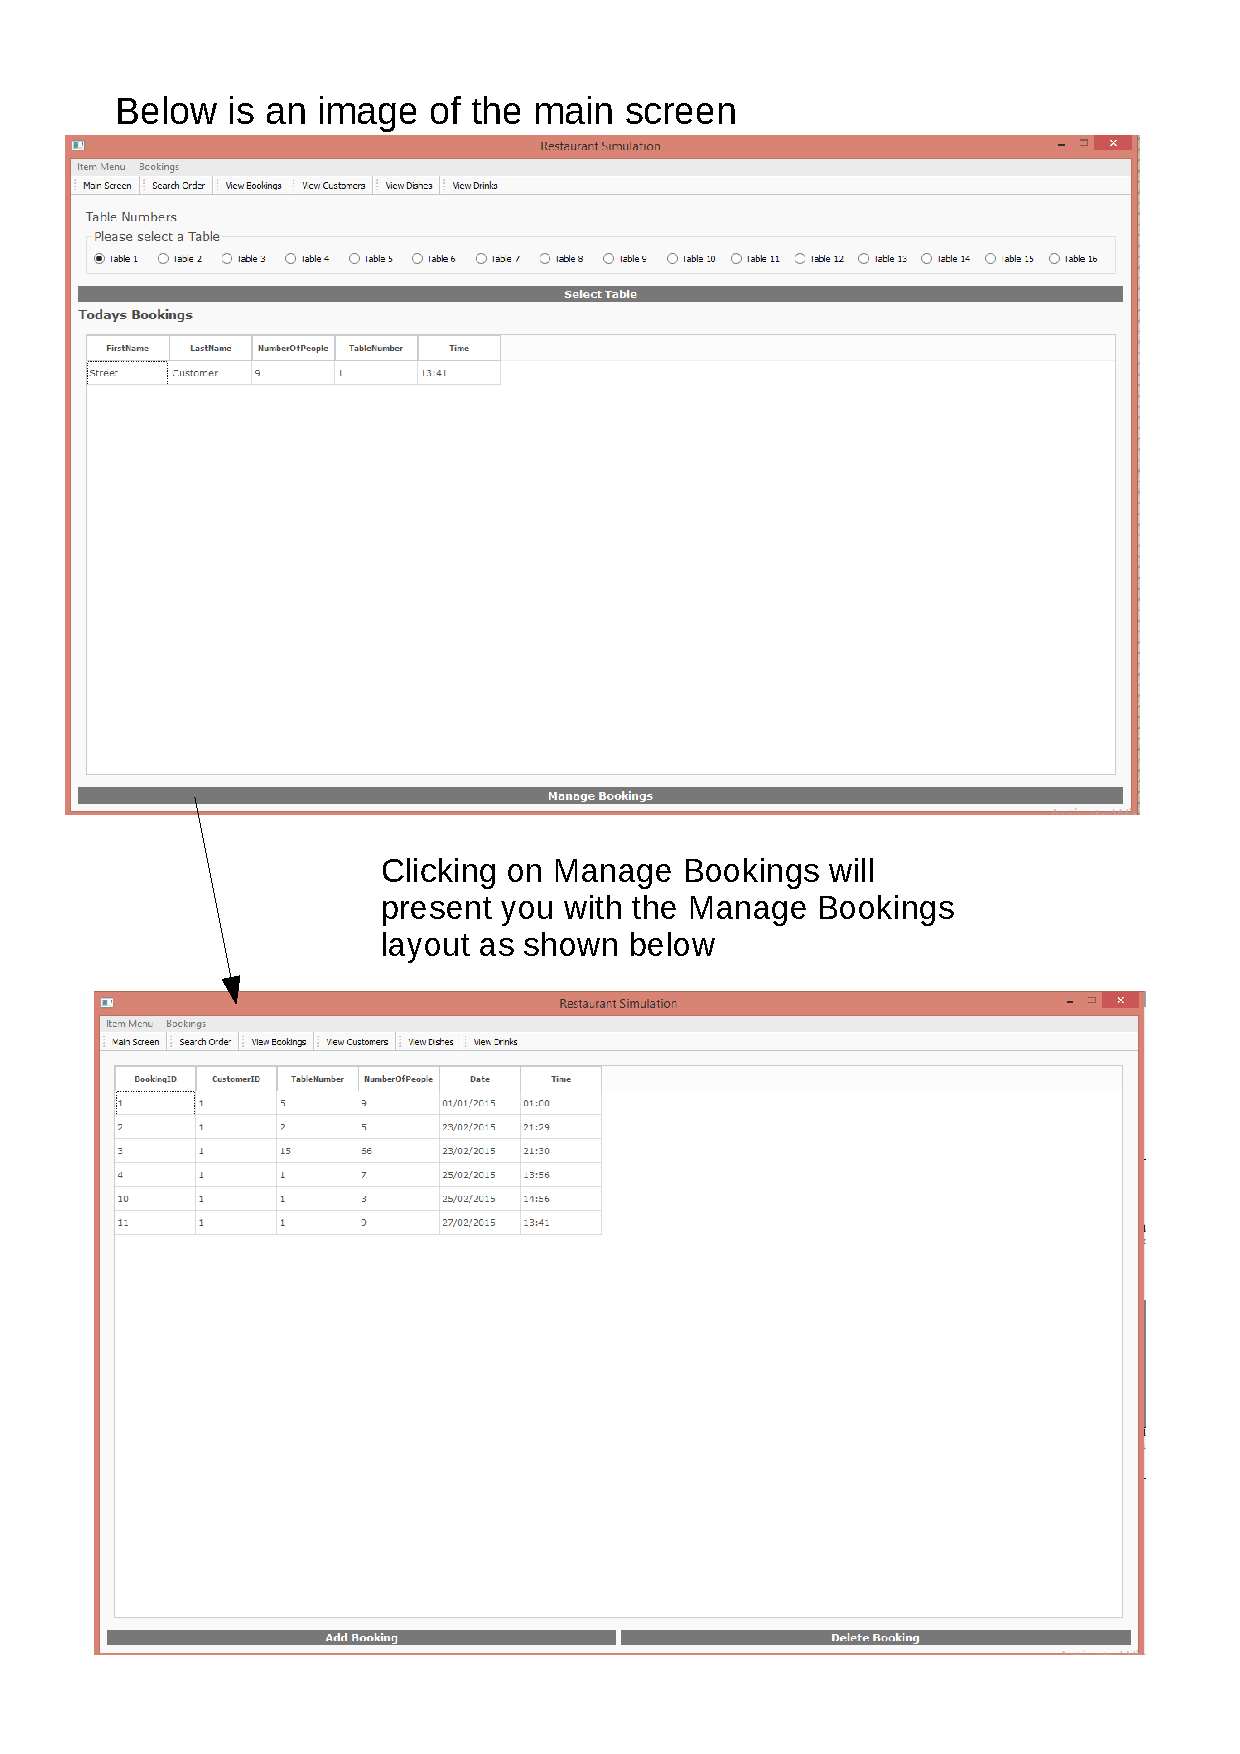
\includegraphics[height = 20cm]{./Testing/images/test1}
    \caption{Manage Booking layout} \label{fig:Test1}
\end{figure}

\subsubsection{Add Booking screen from manage bookings (Test 1.10)}

\begin{figure}[H]
    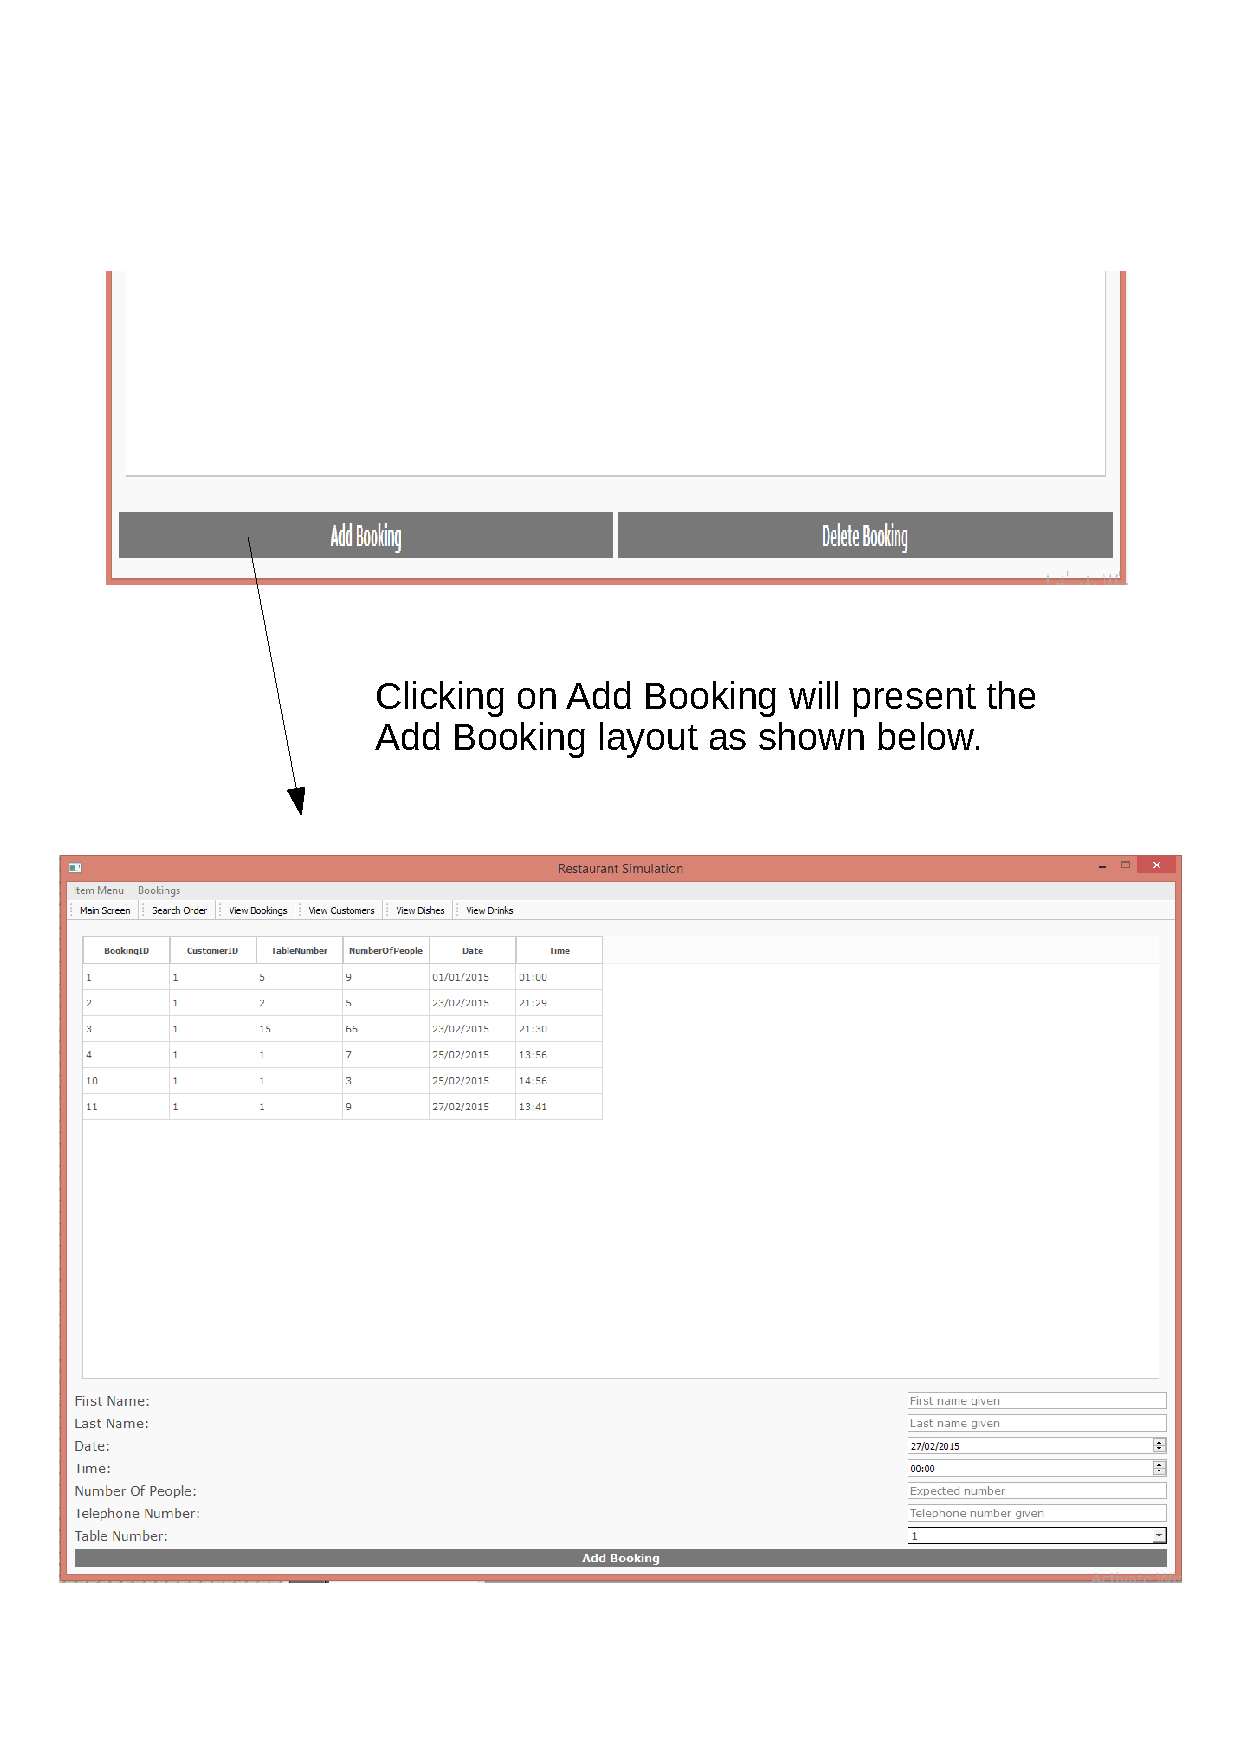
\includegraphics[height = 20cm]{./Testing/images/test2.pdf}
    \caption{Add Booking} \label{fig:Test2}
\end{figure}

\subsubsection{Delete Booking screen from manage bookings (Test 1.13)}

\begin{figure}[H]
    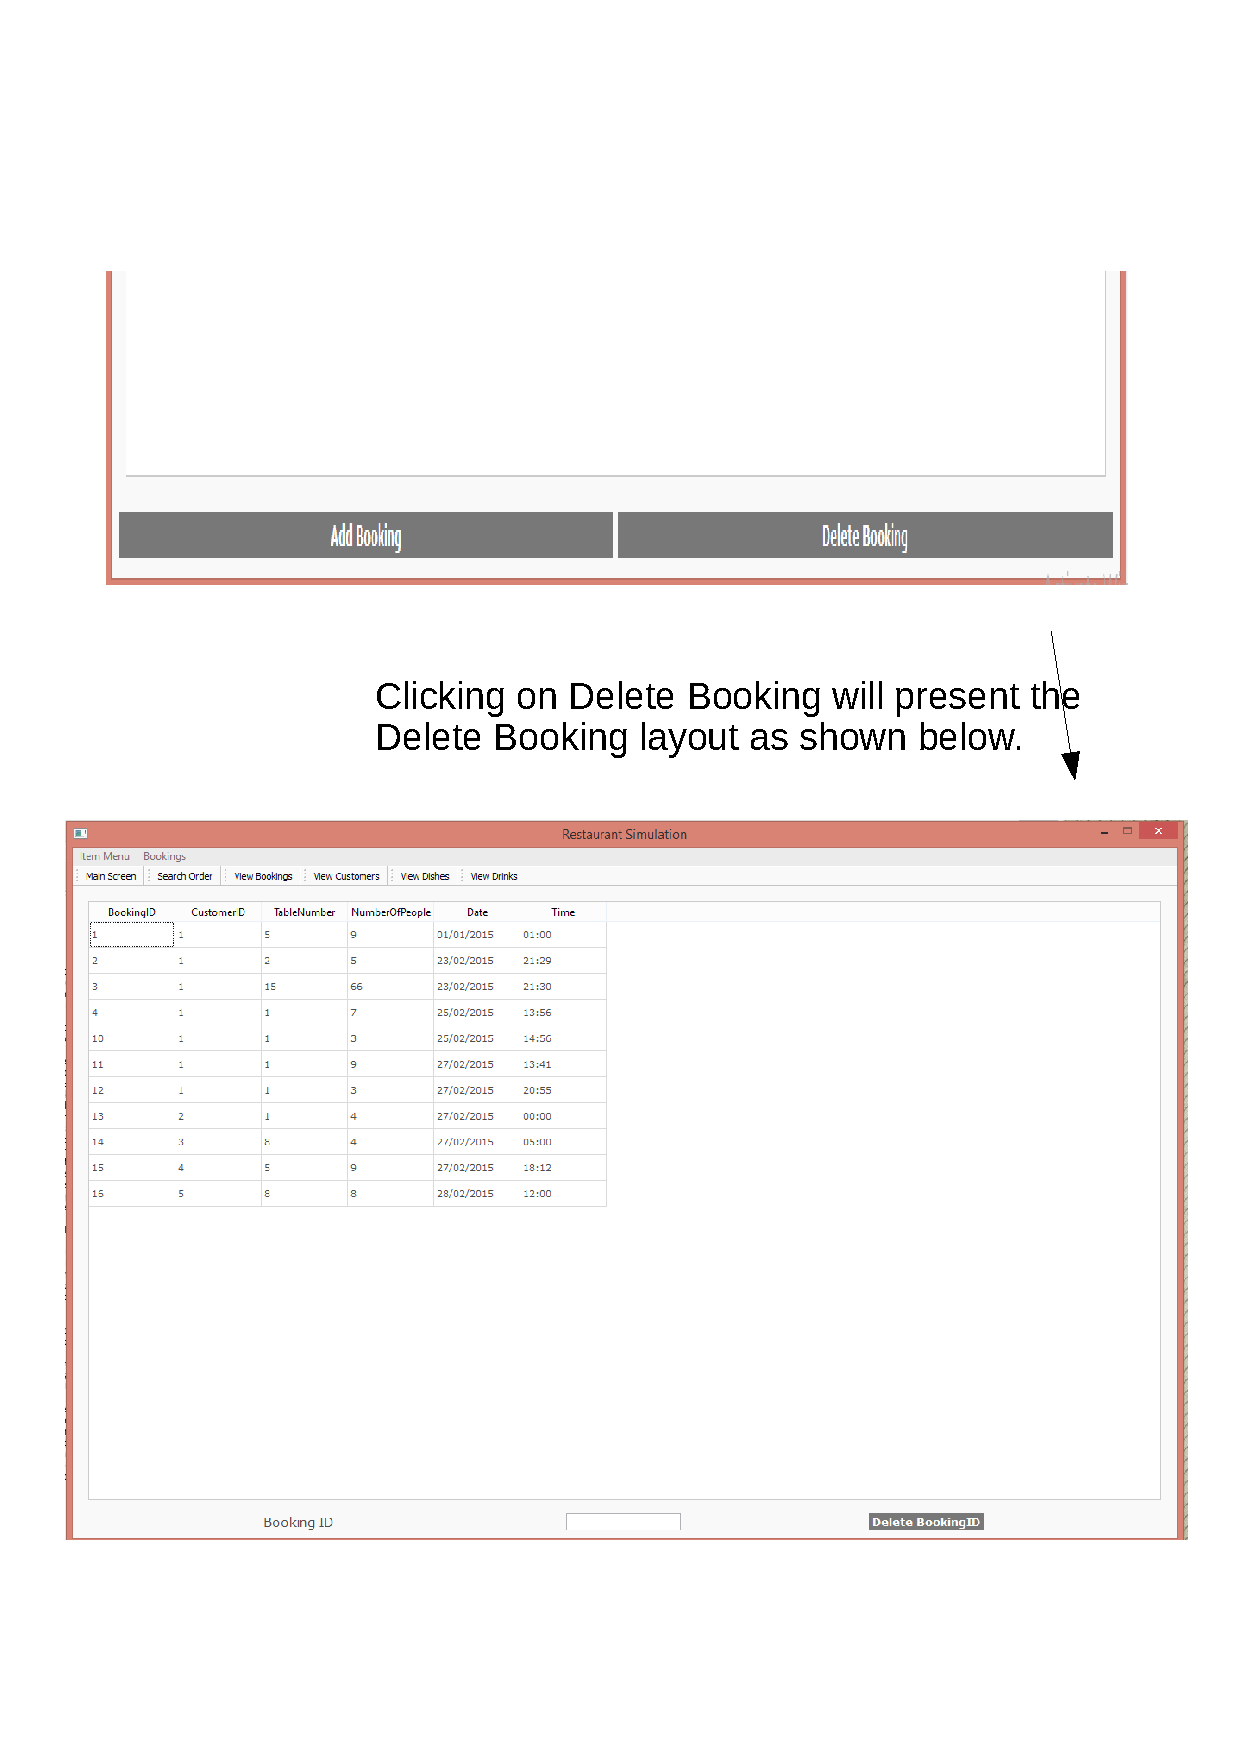
\includegraphics[height = 20cm]{./Testing/images/test3.pdf}
    \caption{Delete Booking layout} \label{fig:Test3}
\end{figure}


\begin{landscape}


\subsubsection{Search Order from tool bar (Test 1.21)}

\begin{figure}[H]
    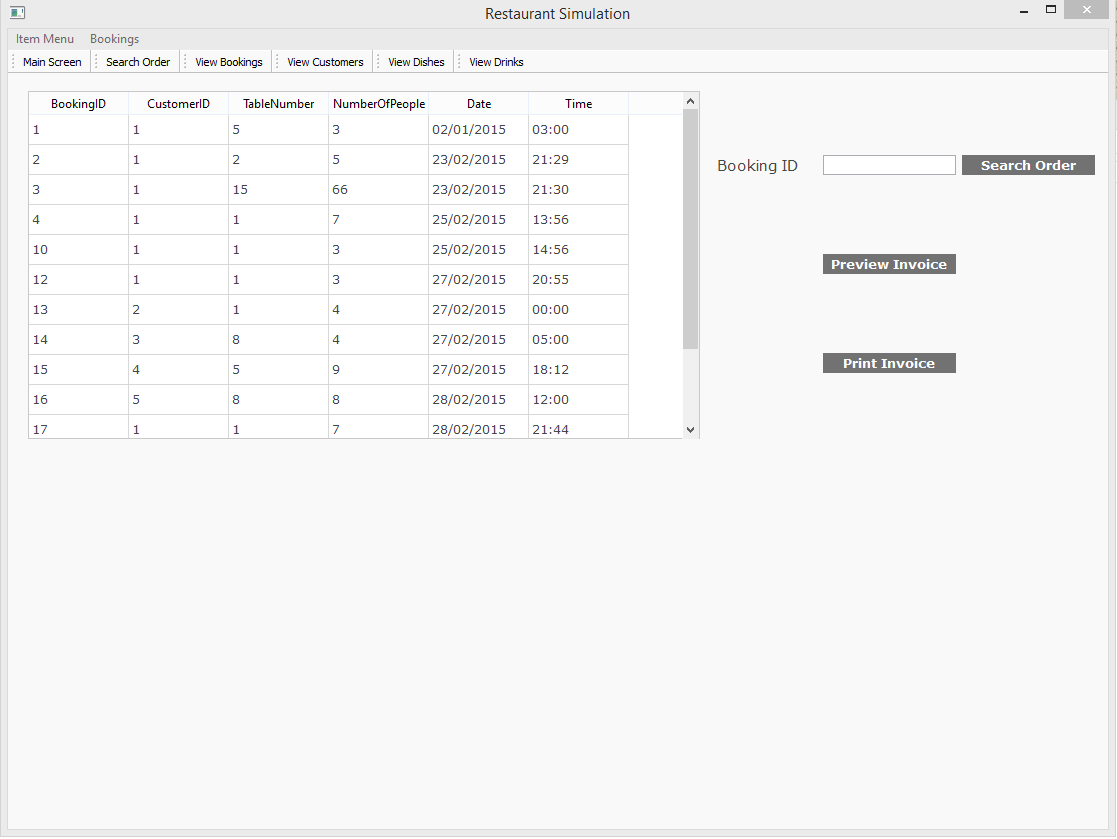
\includegraphics[height = 15cm]{./Maintenance/images/png/screen17}
    \caption{Search Order layout} \label{fig:searchOrder}
\end{figure}

\subsubsection{Assign Customer to table validation (Test 2.04)}

\begin{figure}[H]
    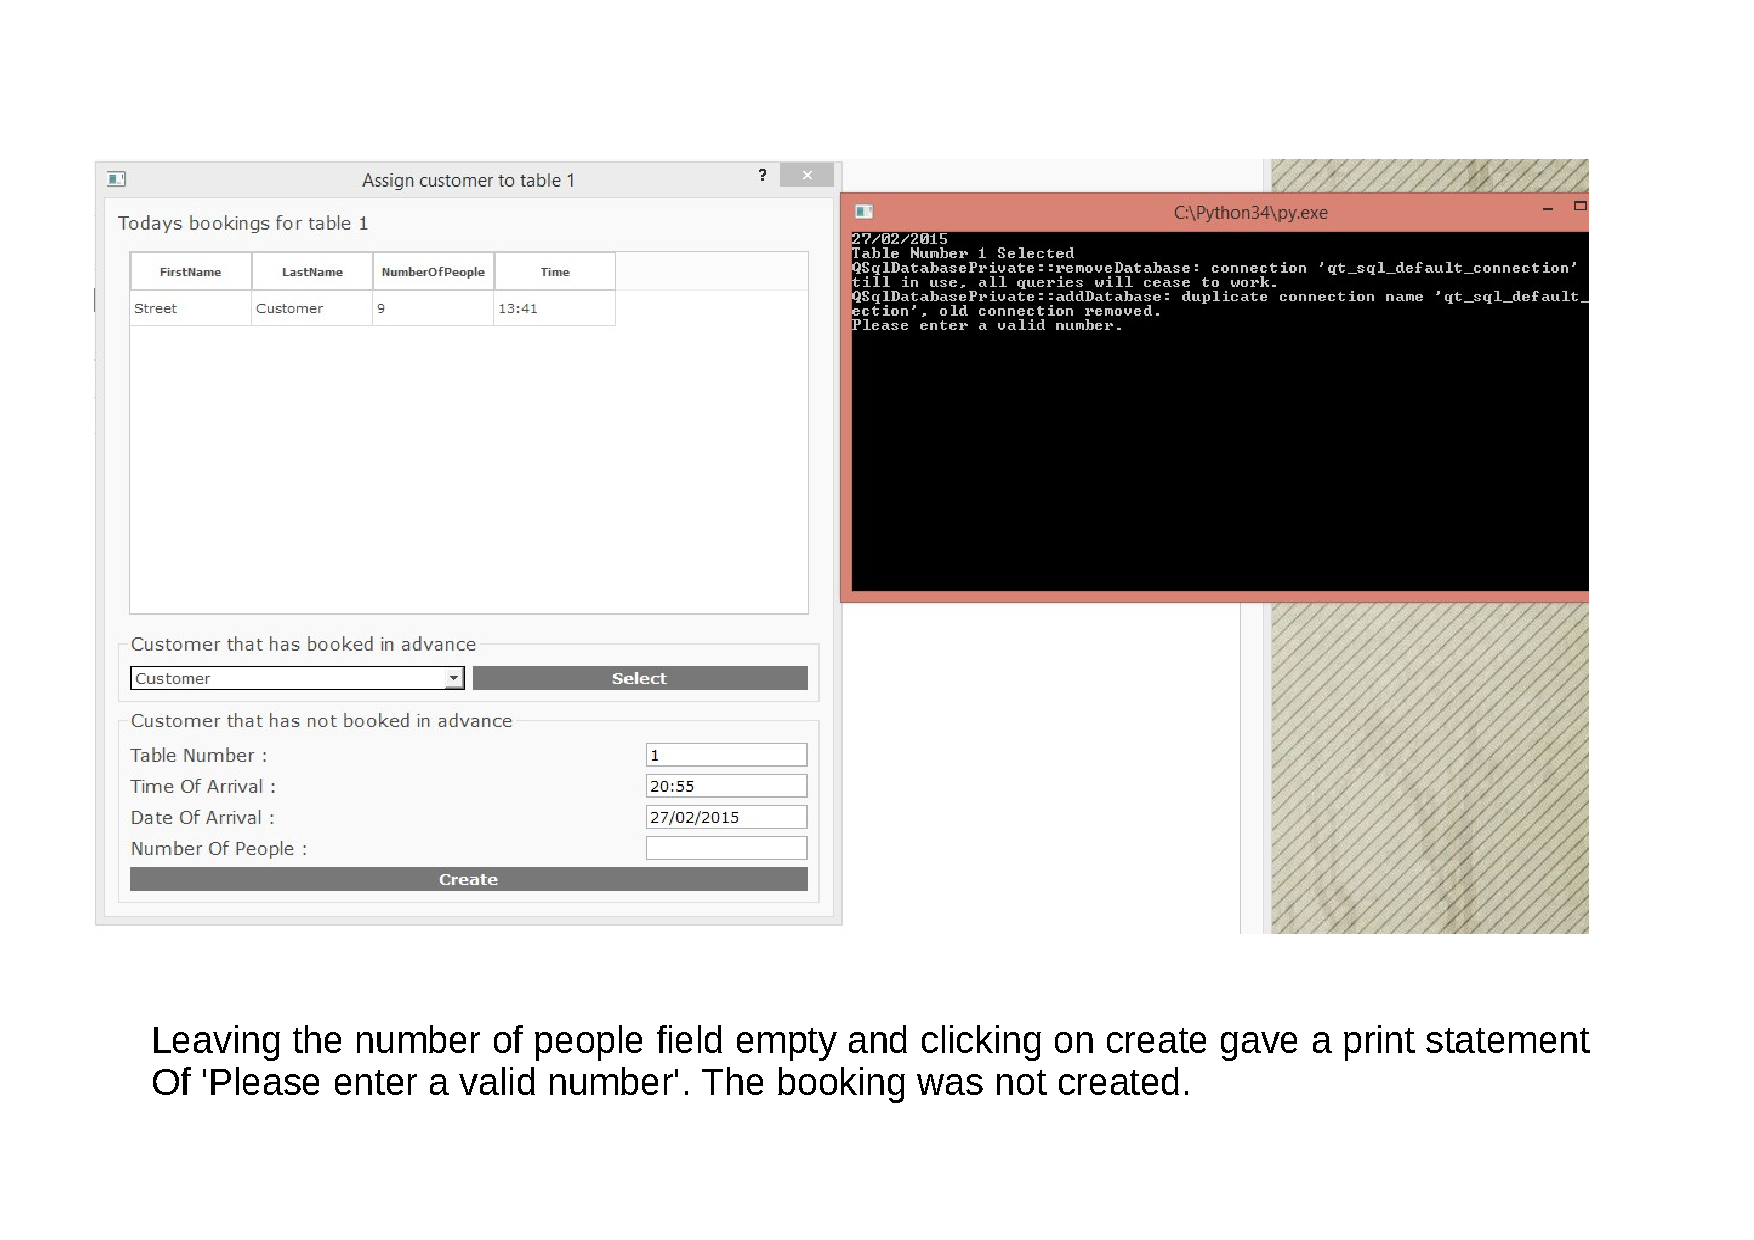
\includegraphics[width = 20cm]{./Testing/images/test4.pdf}
    \caption{Assign customer validation} \label{fig:Test4}
\end{figure}

\subsubsection{Leave Telephone Number field empty error (Test 2.08)}

\begin{figure}[H]
    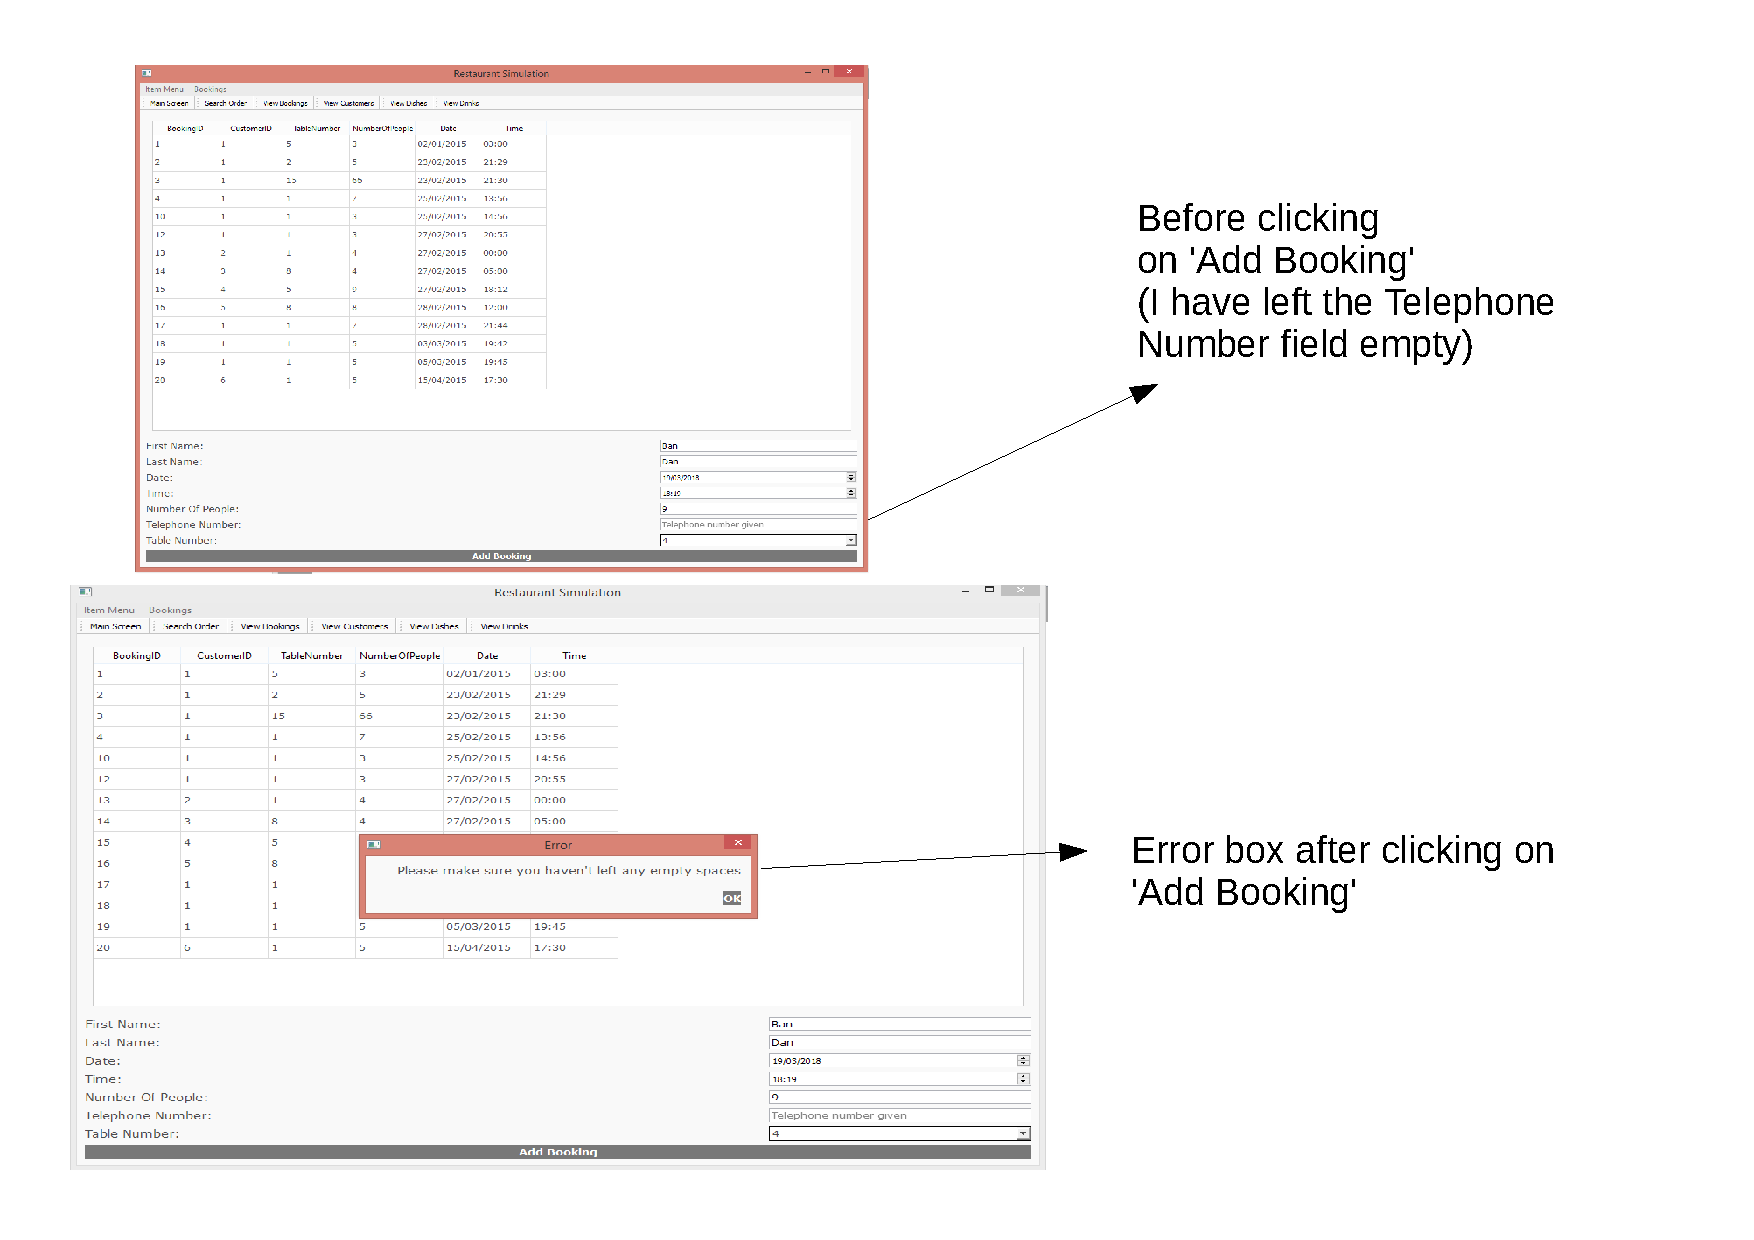
\includegraphics[width = 20cm]{./Testing/images/test12}
    \caption{Error box pop up} \label{fig:Test12}
\end{figure}

\subsubsection{Telephone Number boundary test (Test 2.08.02)}

\begin{figure}[H]
    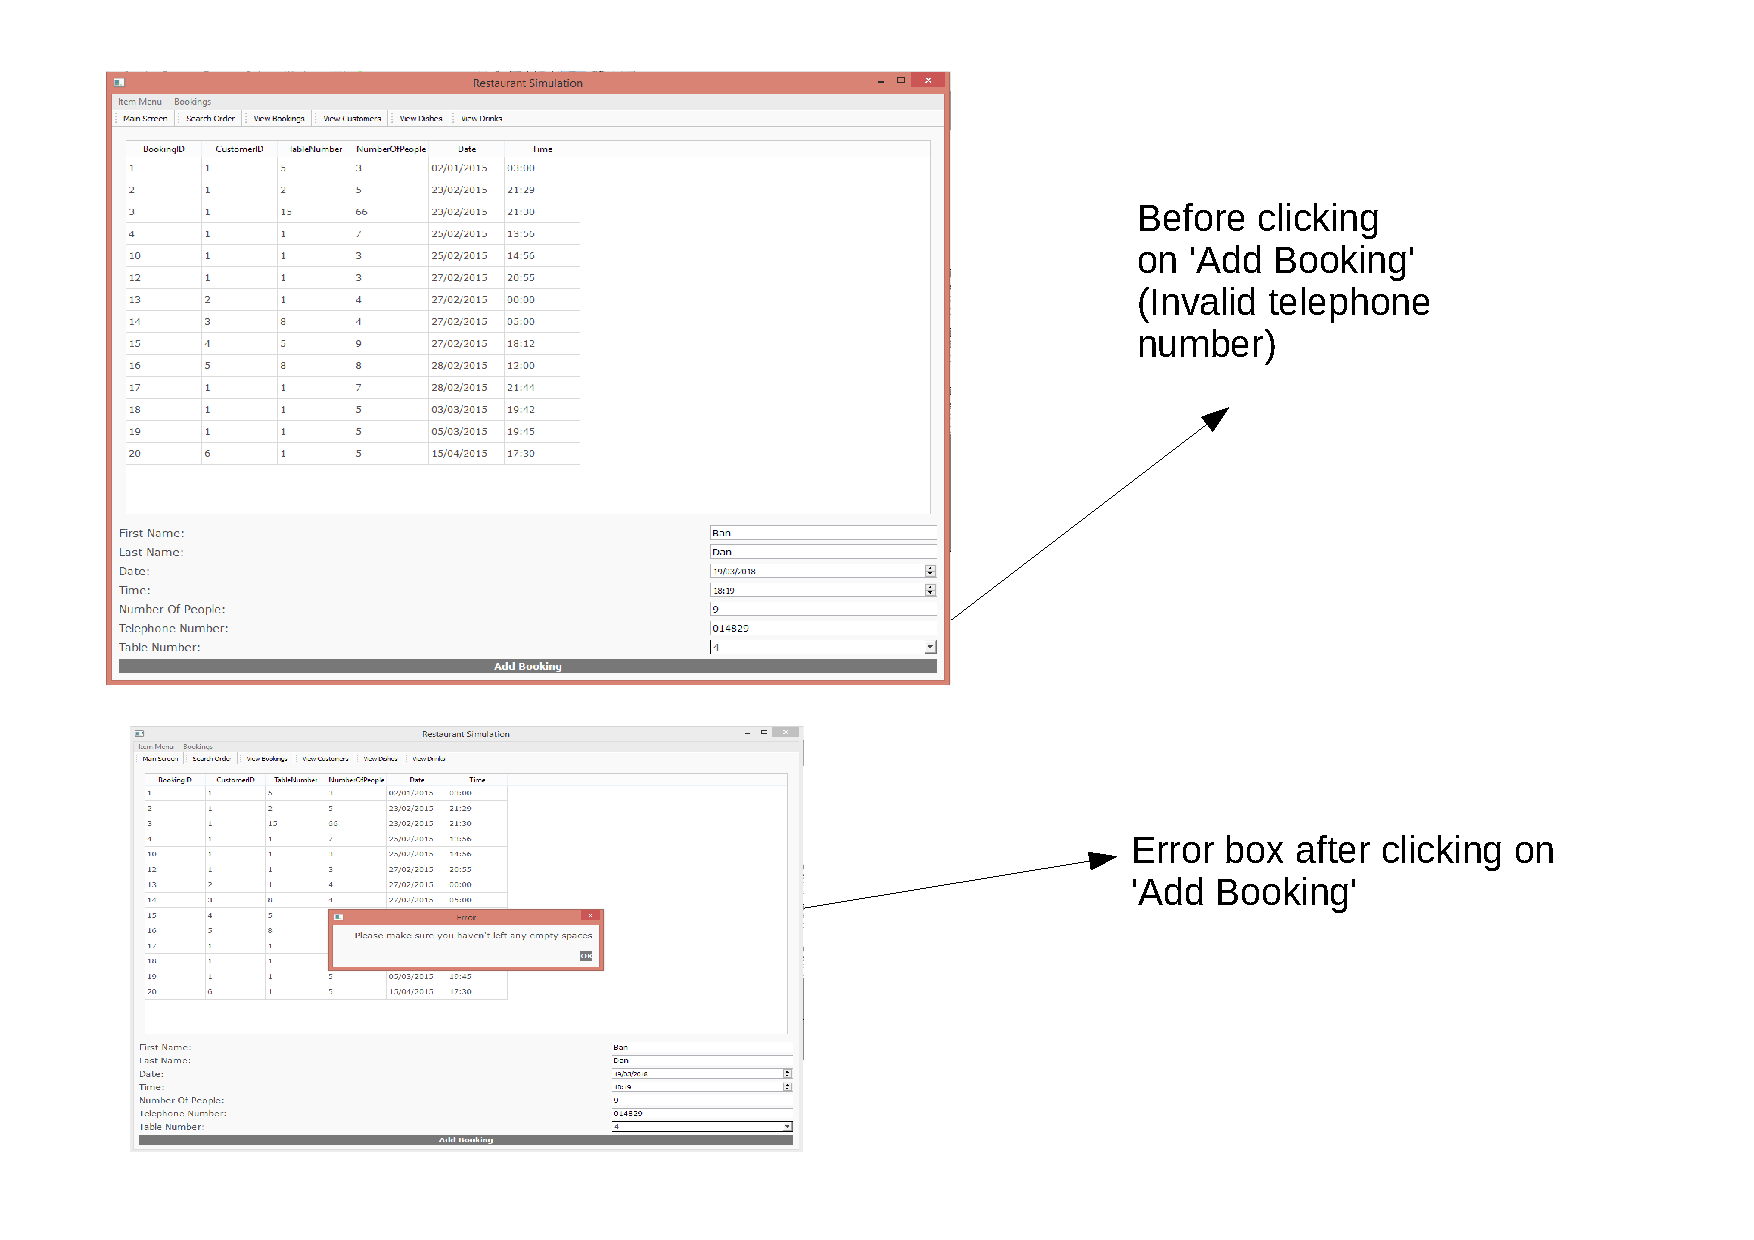
\includegraphics[width = 20cm]{./Testing/images/test13}
    \caption{Error box pop up} \label{fig:Test13}
\end{figure}



\subsubsection{Add Item to Menu verification (Test 2.13.01)}

\begin{figure}[H]
    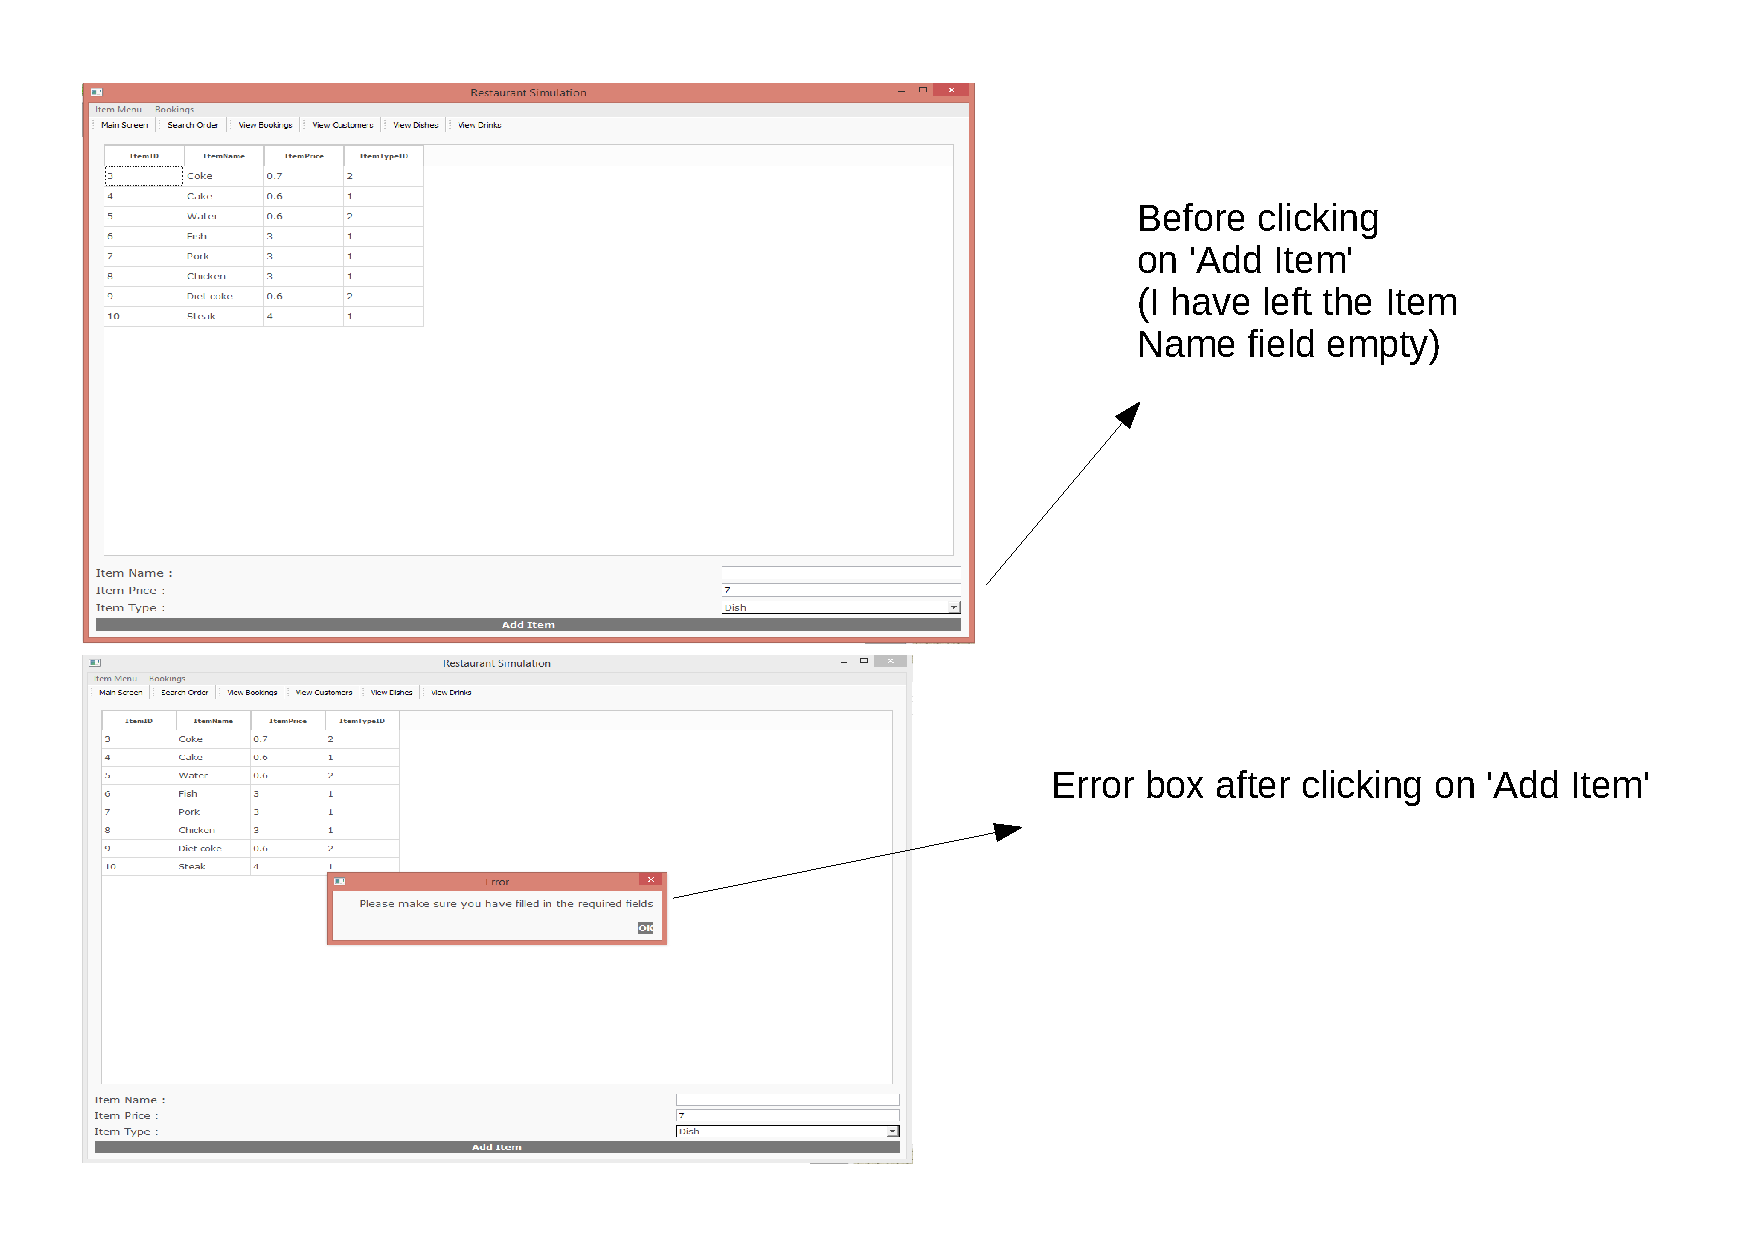
\includegraphics[width = 20cm]{./Testing/images/test11}
    \caption{Item add verification} \label{fig:Test11}
\end{figure}

\subsubsection{Manage Order Box from Assign Customer (Test 3.03) }

\begin{figure}[H]
    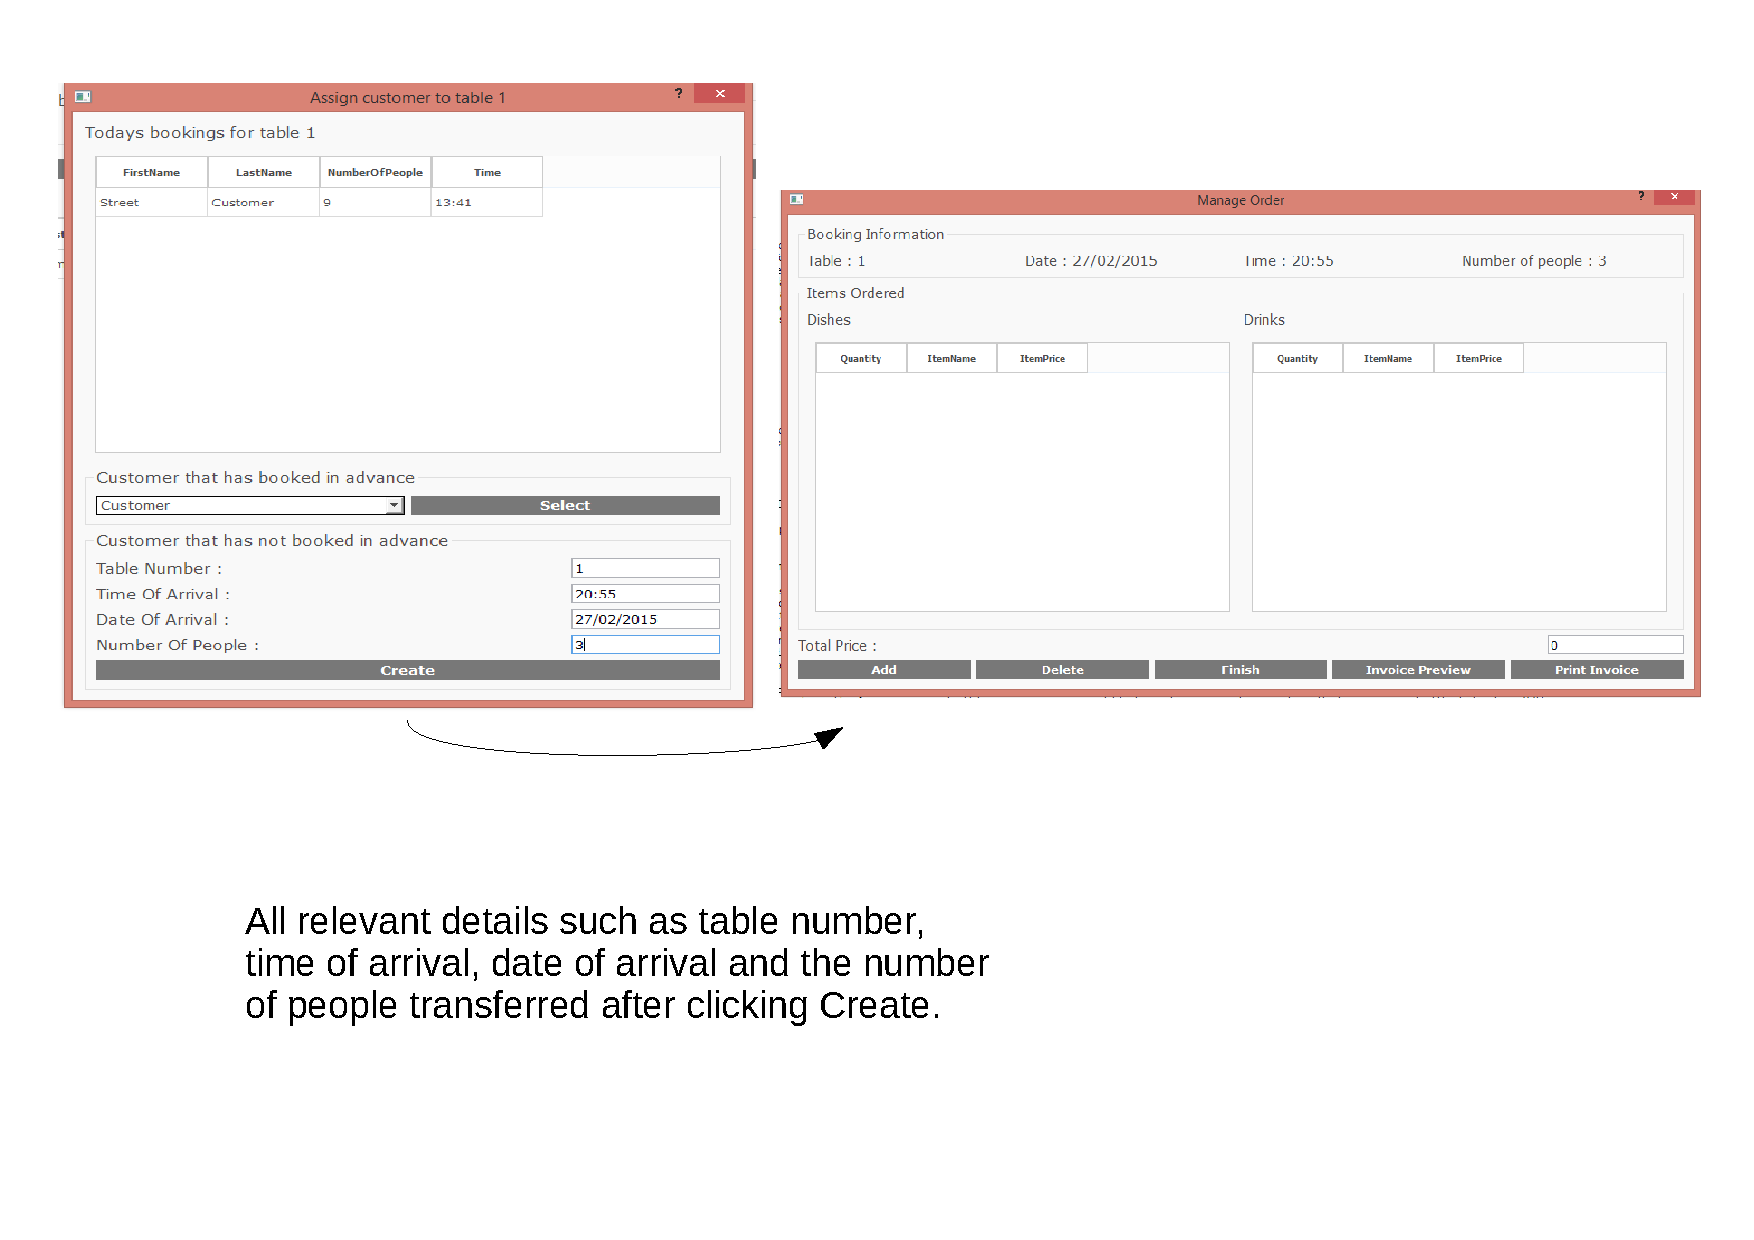
\includegraphics[width = 20cm]{./Testing/images/test5.pdf}
    \caption{Check all details transferred} \label{fig:Test5}
\end{figure}

\subsubsection{Select function from Assign Customer (Test 3.04)}

\begin{figure}[H]
    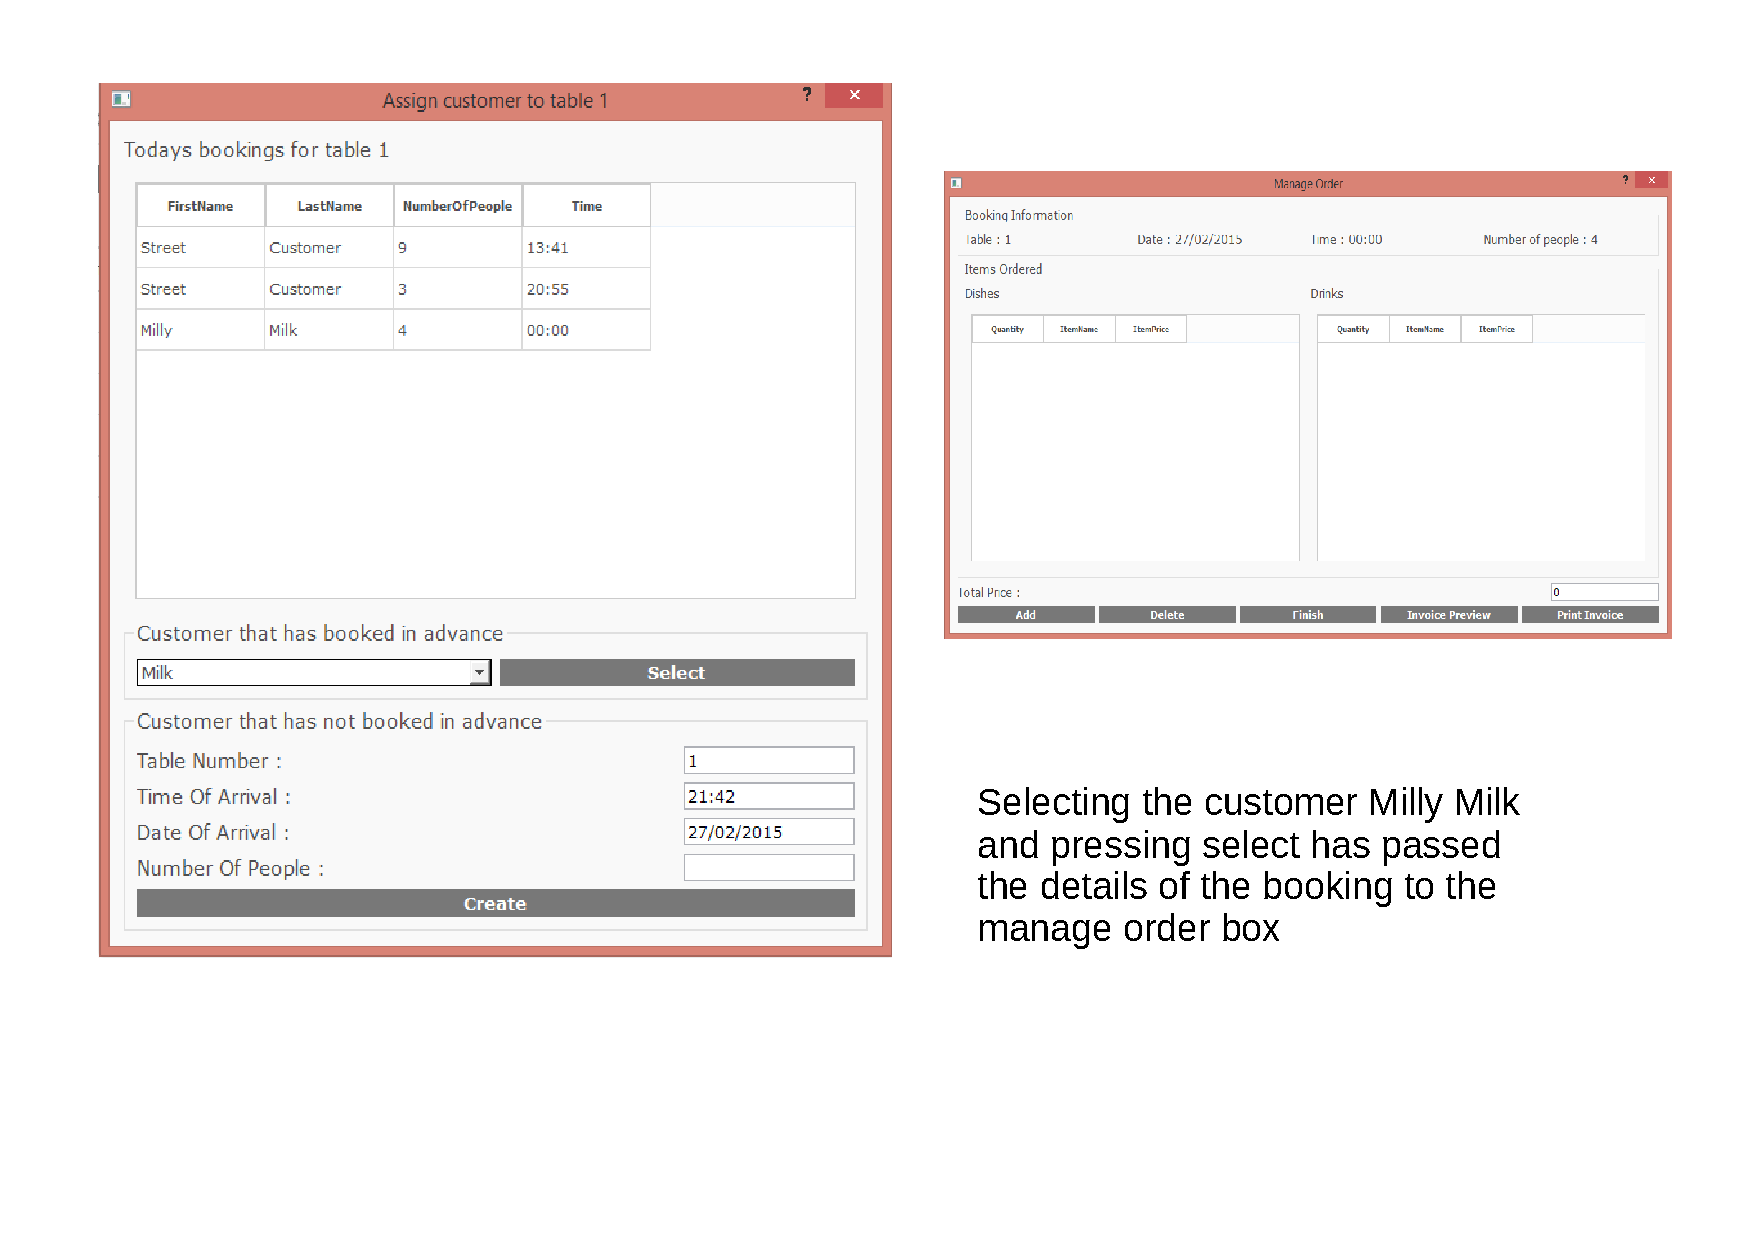
\includegraphics[width = 20cm]{./Testing/images/testt1.pdf}
    \caption{Check the select function works ( passes the correct details of the selected customer)} \label{fig:Test8}
\end{figure}

\subsubsection{Total Price Update (Test 4.03)}

\begin{figure}[H]
    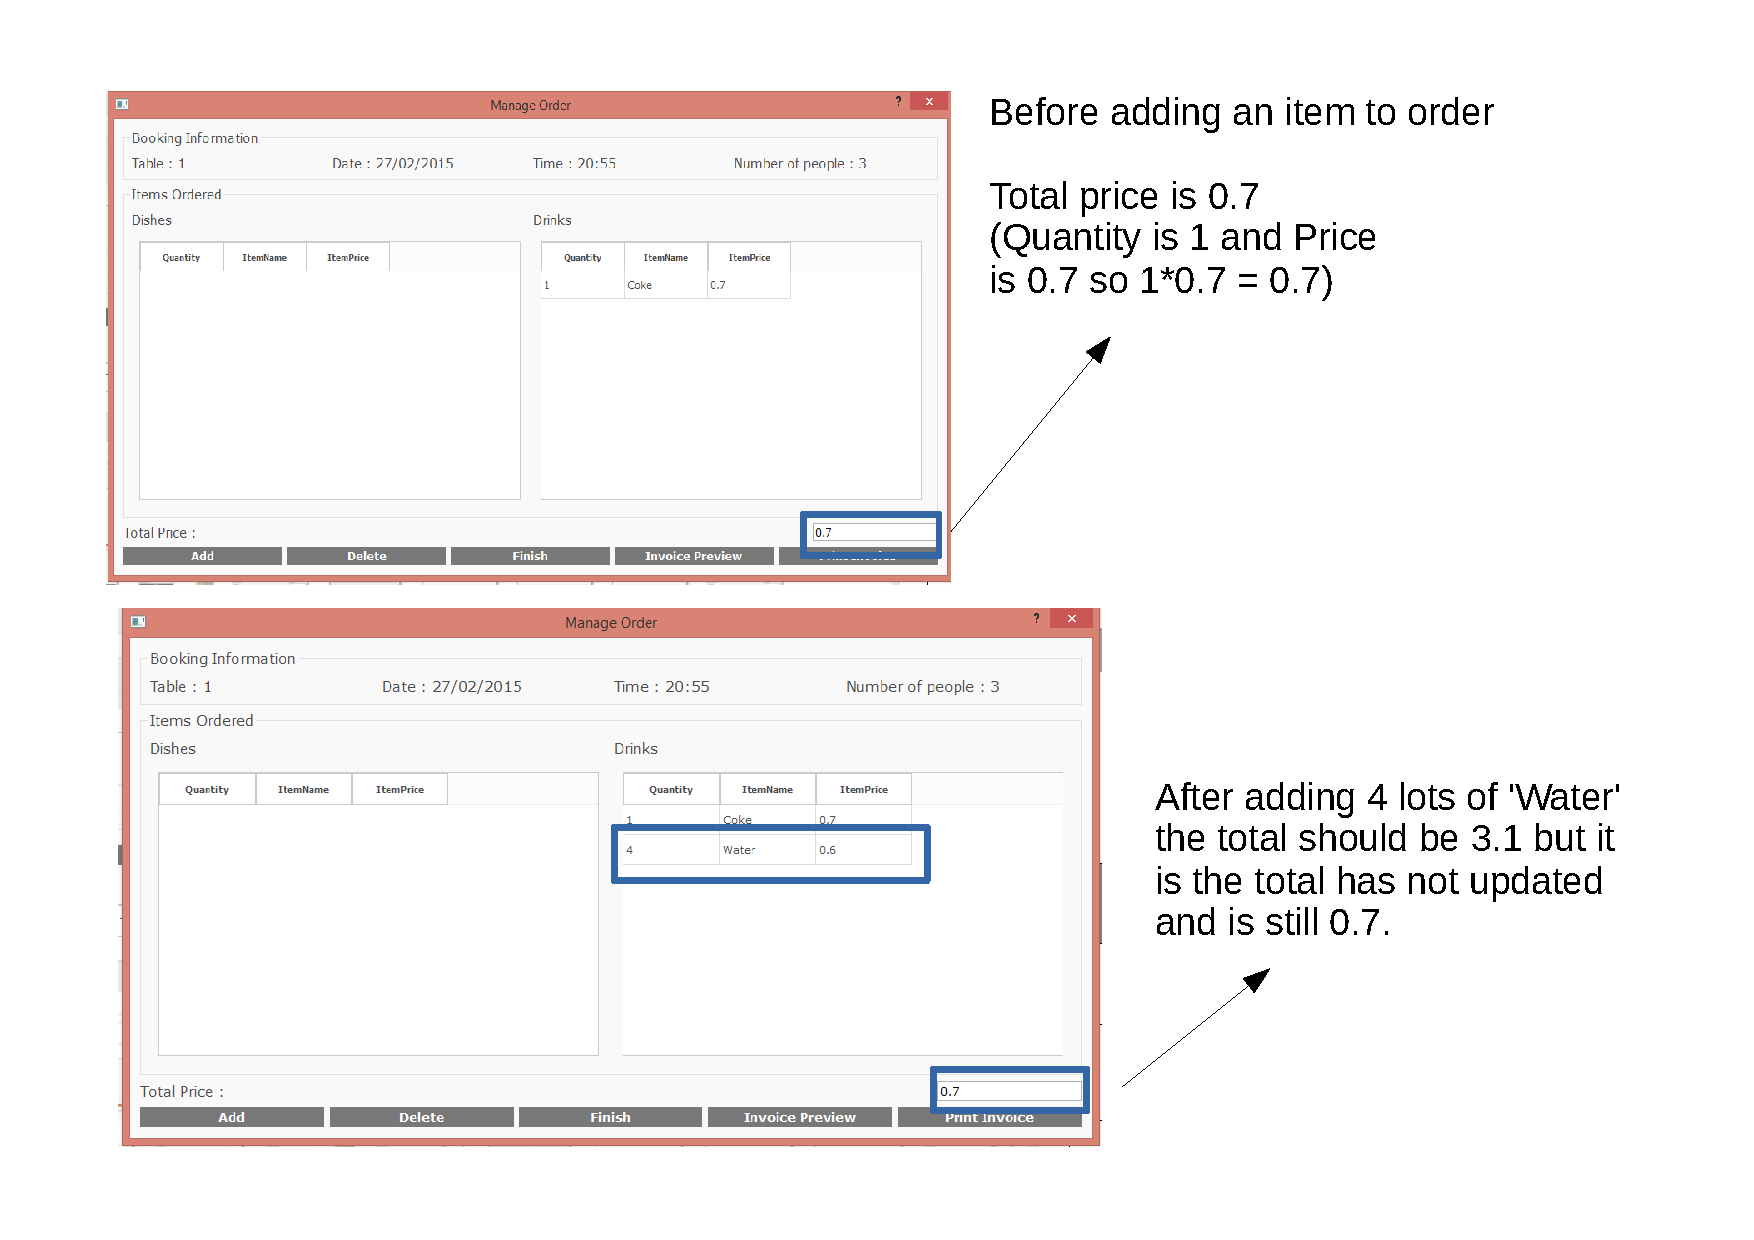
\includegraphics[width = 20cm]{./Testing/images/test10}
    \caption{Total Price does not update at the manage order box after adding item} \label{fig:Test10}
\end{figure}

\subsubsection{Increase Quantity Check (Test 4.05)}

\begin{figure}[H]
    \includegraphics[width = 20cm]{./Testing/images/Test6.pdf}
    \caption{Quantity check} \label{fig:Test6}
\end{figure}

\subsubsection{Checking if booking \& customer details has stored correctly (Test 4.09) } 

\begin{figure}[H]
    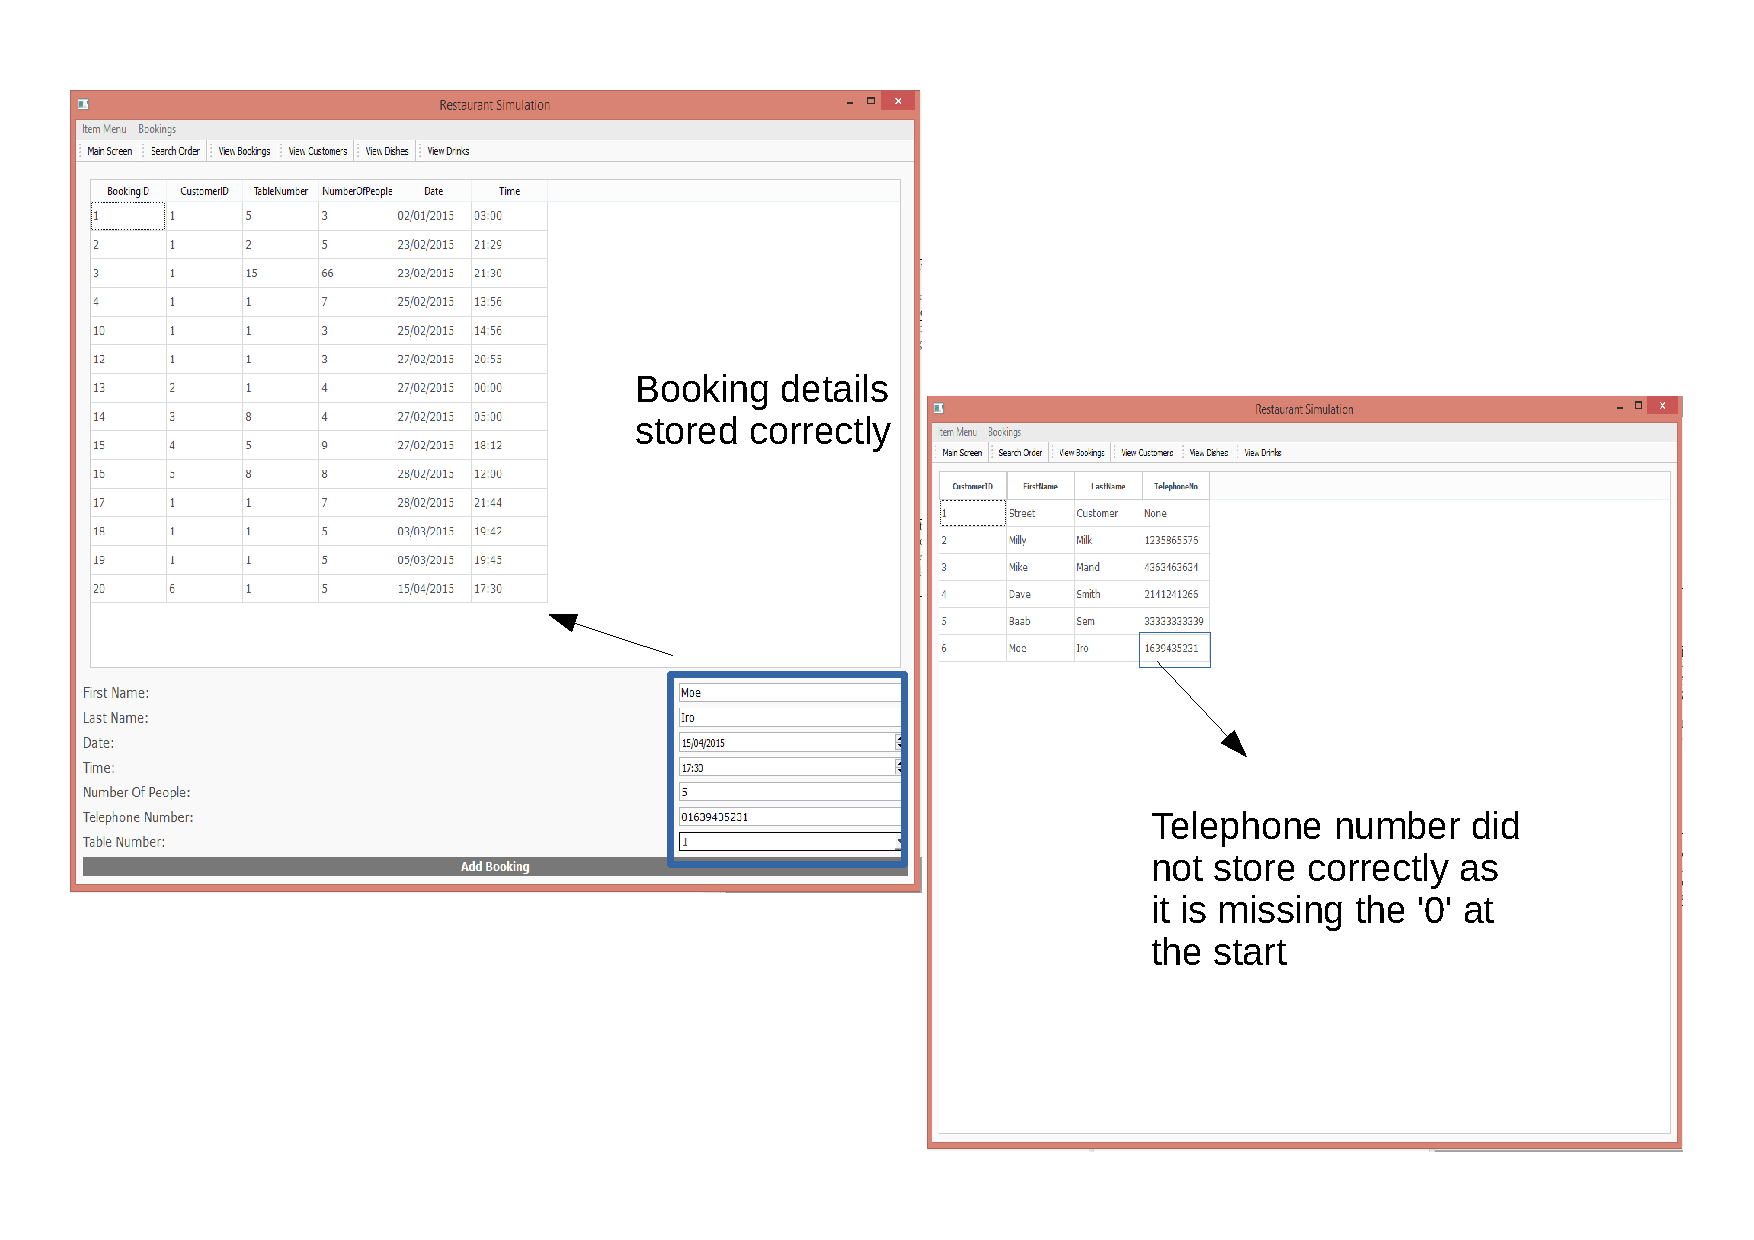
\includegraphics[width = 20cm]{./Testing/images/test9}
    \caption{Adding a booking also creates a new customer record} \label{fig:Test9}
\end{figure}

\subsubsection{Invoice Preview (Test 1.32 \& 3.05)}

\begin{figure}[H]
    \includegraphics[width = 20cm]{./Testing/images/Test7.pdf}
    \caption{Invoice check} \label{fig:Test7}
\end{figure}

\subsubsection{Search Order tab from tool bar (Test 4.08.02)}

\begin{figure}[H]
    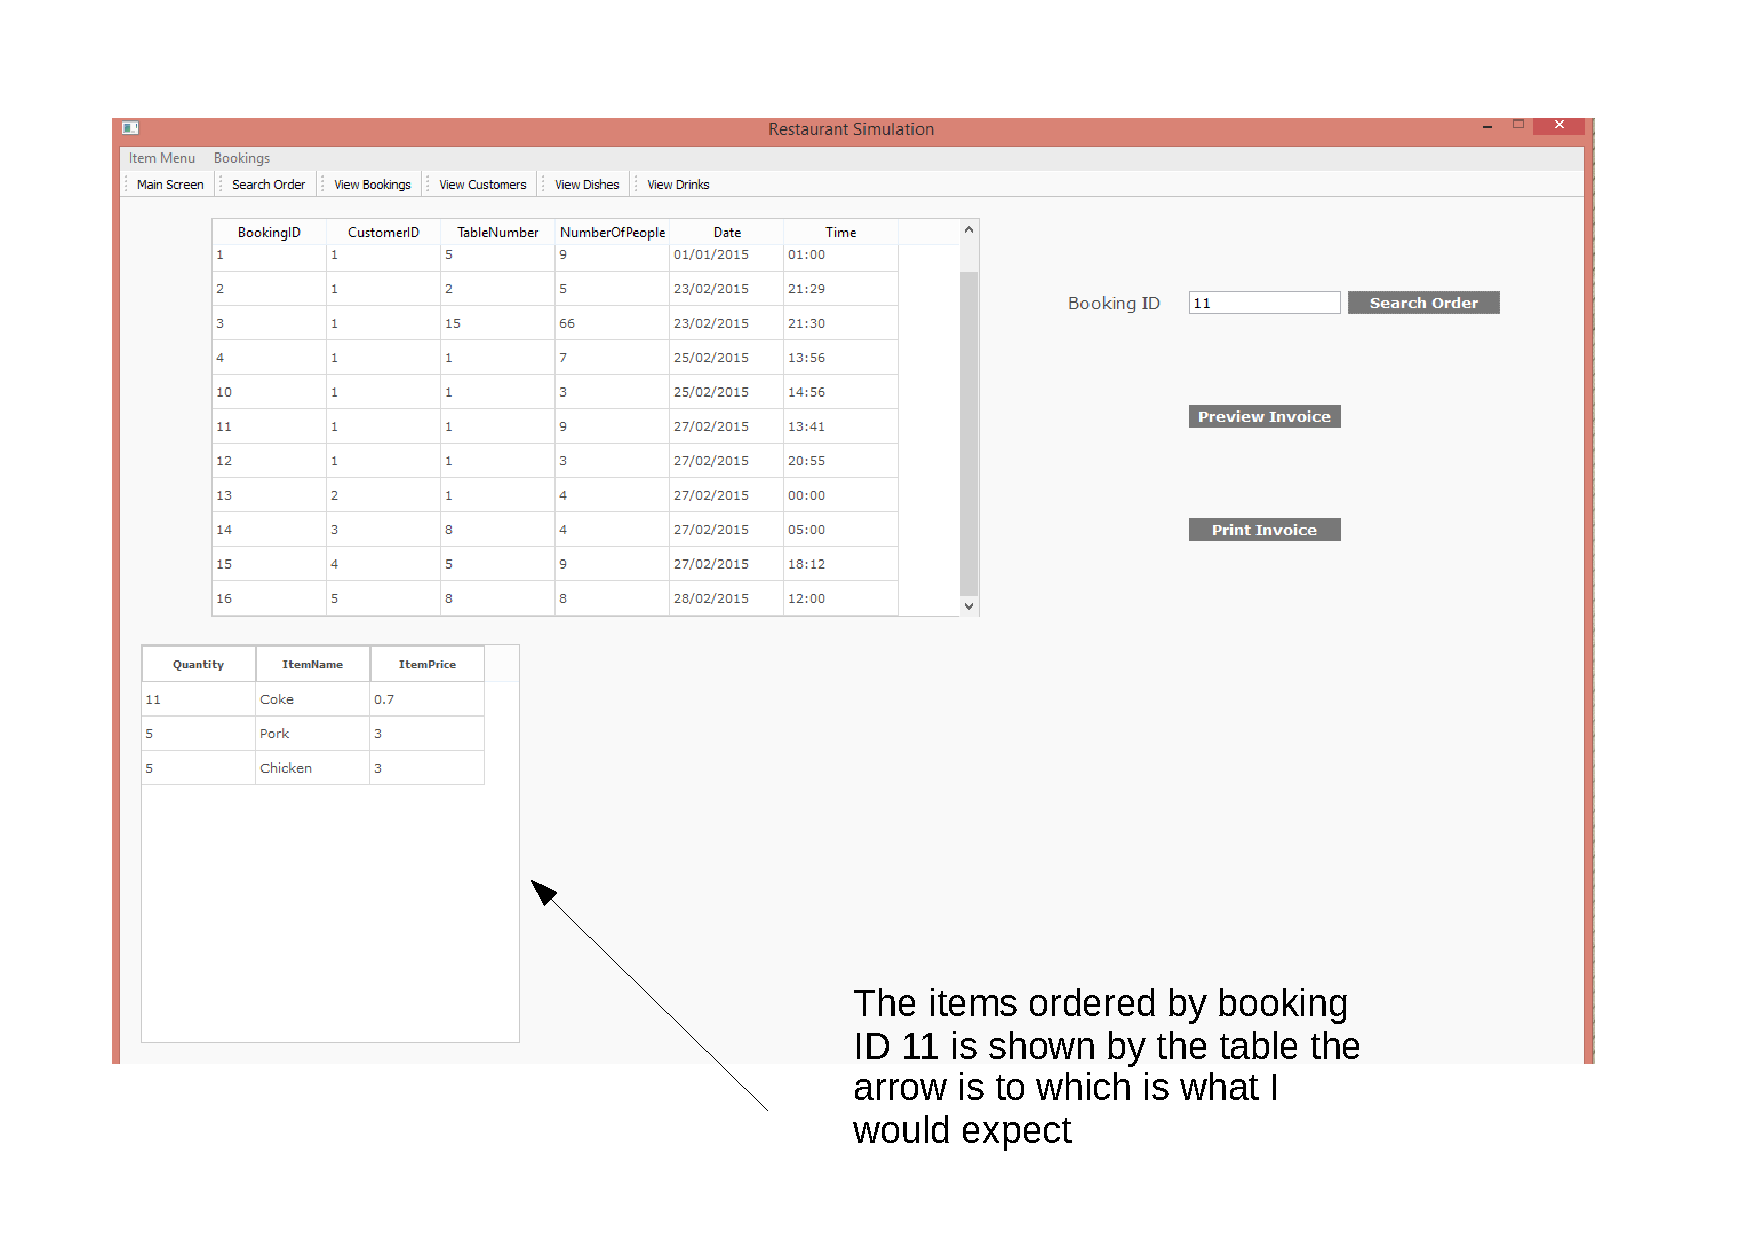
\includegraphics[width = 20cm]{./Testing/images/booking11.pdf}
    \caption{Checking the search function} \label{fig:searchFunction}
\end{figure}

\subsubsection{Referential Integrity test relating the deletion of a booking (Test 6.03)}

\begin{figure}[H]
    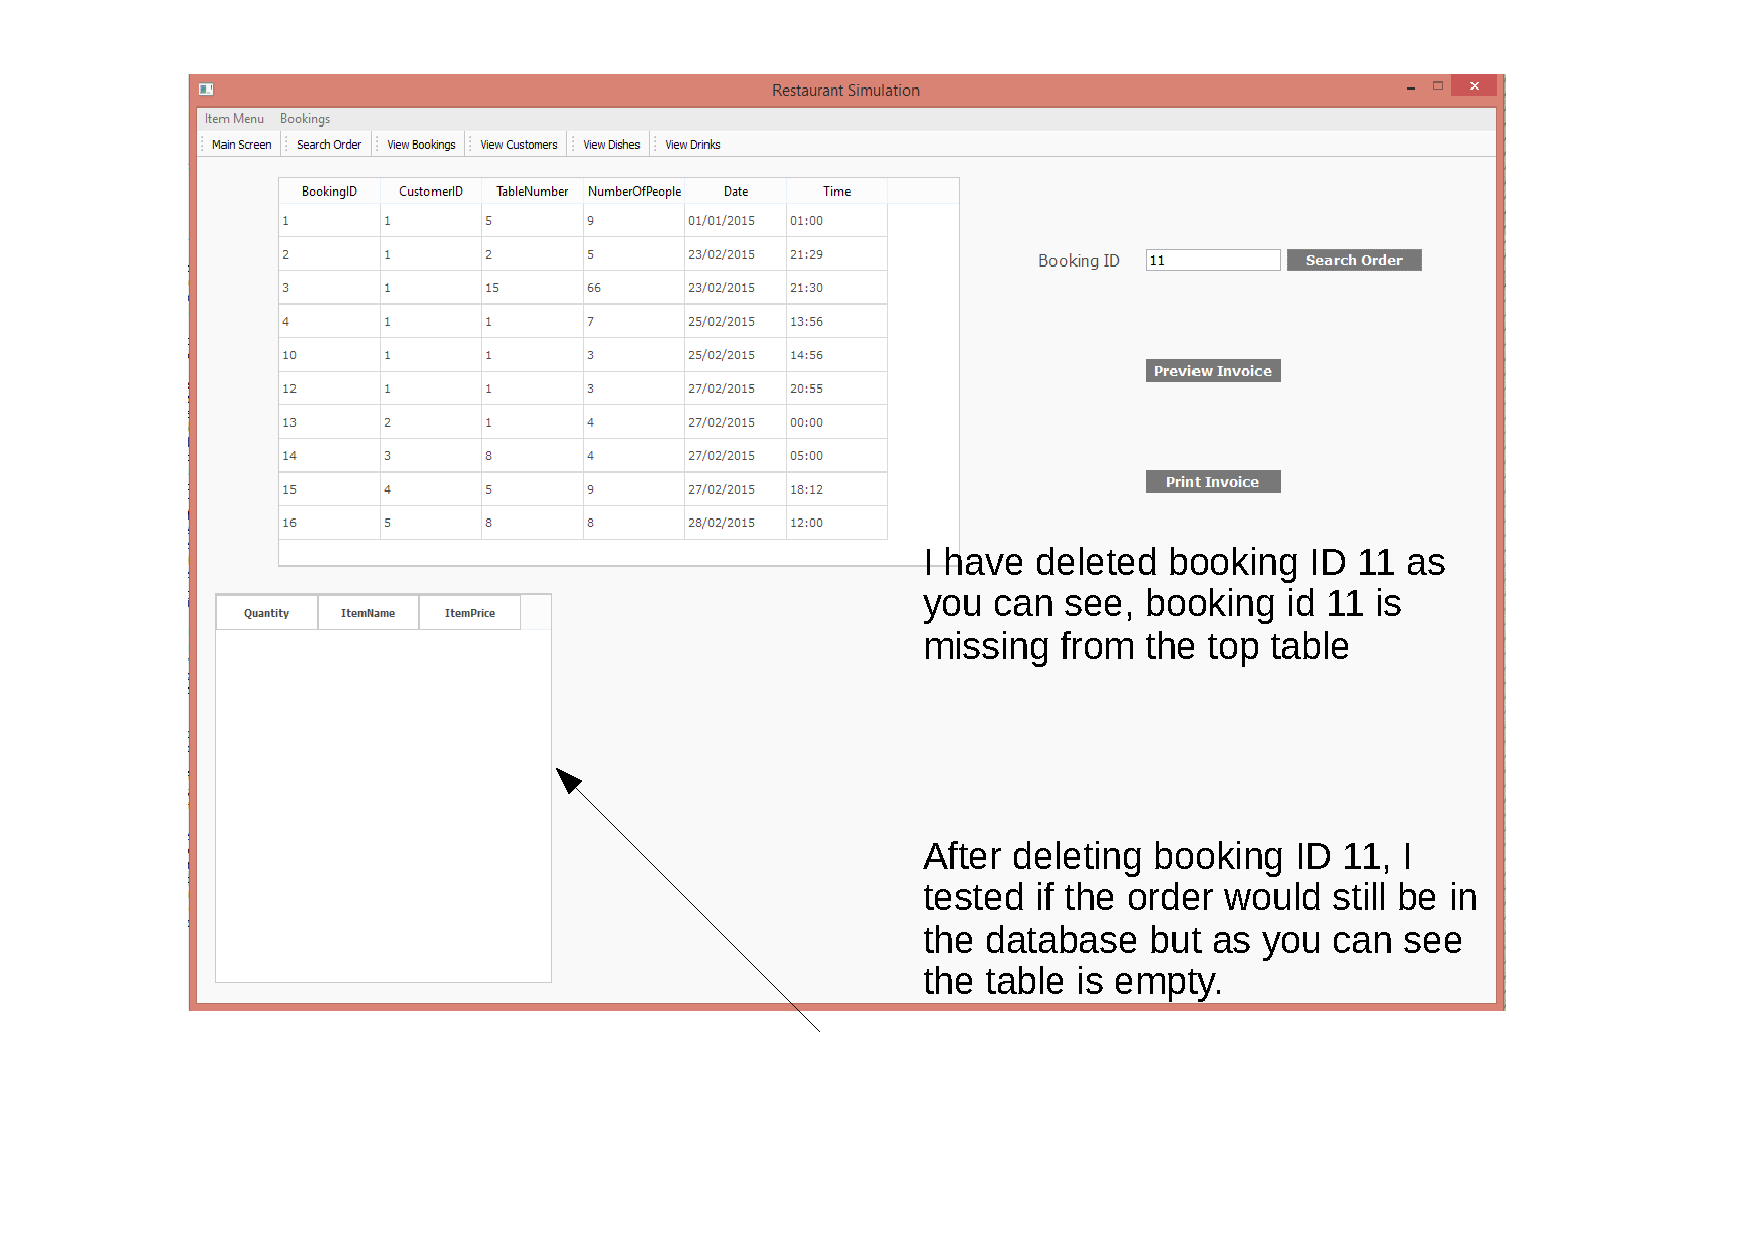
\includegraphics[width = 20cm]{./Testing/images/booking11delete.pdf}
    \caption{Checking if the order is deleted after deleting booking ID 11} \label{fig:searchDeletedBooking}
\end{figure}






\end{landscape}

\section{Evaluation}

\subsection{Approach to Testing}


I made sure I tested my program thoroughly by going through different types of testing strategies. Going through different testing strategies made me cover most, if not all areas of my program such as testing the flow of control, validation, algorithms and the outputs.  I chose this approach to ensure my whether my program was usable or not. My first strategy (series 1) was top-down testing which enabled me to test the effectiveness of the navigation in the application. Series 2.

I made sure I tested my program thoroughly by going through different types of testing strategies. Going through different testing strategies made me cover most, if not all areas of my program such as testing the flow of control, validation, algorithms and the outputs.  I chose this approach to ensure my whether my program was usable or not. My first strategy (series 1) was top-down testing which enabled me to test the effectiveness of the navigation in the application. Series 2 is made up of bottom-up testing to ensure that the validation in the application is functioning as intended. Series 3 is made up of black-box testing to make sure the data in my program is being passed/stored correctly and series 4 is made up of white-box testing to make sure that the algorithms used are producing the correct output. As for series 5, it is the acceptance testing to get an overall idea if the application matches my client's specification. The last test series (test series 6) is made up of integration tests to ensure that the data in the database is consistent.


\subsection{Problems Encountered}

I encountered a problem on test 4.03 (\ref{fig:Test10} on page \pageref{fig:Test10}) . The total price did not refresh after adding an item, it would only refresh after closing the manage order box and selecting the table again. I also experienced a problem on test 4.09 (\ref{fig:Test9} on page \pageref{fig:Test9}) where all the details of the booking correctly stored in the database apart from the telephone number. The telephone number stored the telephone number input however, if 0 was the first number, the 0 would not be stored but the rest of the numbers would.

\subsection{Strengths of Testing}

The strengths of the approach I took were that I was able to find out whether my program was usable or not by testing each component of the system using the different test strategies (See page 88 for the testing strategies). Users of my system will undoubtly make mistakes when inputting information and so I have tested different types of test data which proved that my system can be reliable in that prospect (See test series 2) . In addition, checking the flow of control proved the navigation of the system to be effective.

\subsection{Weaknesses of Testing}

When I tested the sql statements, I relied on the tables displayed on my application to tell me whether the sql statements worked without problems. For example, I deleted a booking on test 6.03 (\ref{fig:searchDeletedBooking} on page \pageref{fig:searchDeletedBooking}) and checked to see if there was an order attached to the booking. The order did not display after searching for the booking but it may have still been in the database - which is what I didn't check. Also, the applcation has 16 radio buttons that represent the tables in the restaurant - I did not test all of them which would of meant that there could have been a fault with the application within the radio buttons that I did not test. Moreover, I did not test on what would happen if I added relatively the same record twice. For example, adding an item to the menu called 'Pork' with a price of 5.3 and then adding 'Pork' again with a price of 4.3 . This would cause confusion after adding lots of records to the database. 

\subsection{Reliability of Application}

I believe that the application is reliable. I have tested the input validation which worked as the system did not proceed if there was an invalid input which would mean there couldn't be any faulty data in the database. Examples of validation can be found on tests 2.08(\ref{fig:Test12} on page \pageref{fig:Test12}) , 2.08.02 (\ref{fig:Test13} on page \pageref{fig:Test13}) and 2.13.01 (\ref{fig:Test11} on page \pageref{fig:Test11}) . However, it would be up to the User to input the correct data such as correctly spelling an item when adding an item to the menu or inputting the right ID when deleting a record.


\subsection{Robustness of Application}

After testing my system without closing it, I believe that application is robust as I did not experience any crashes or any problems that made me not be able use the application normally. Testing the validation did not affect the application in anyway, same goes for the execution of the sql queries.

After testing my system without closing it, I believe that application is robust as I did not experience any crashes or any problems that made me not be able use the application normally. Testing the validation did not affect the application in anyway, same goes for the execution of the sql queries.An example of me testing the validation can be found on figure \ref{fig:Test1} on page \pageref{fig:Test12}.

